% !TEX program = xelatex
\documentclass[UTF8,fontset=fandol,a4paper,11pt]{ctexart}
\usepackage[margin=21mm,top=23mm,bottom=22mm,headheight=16pt]{geometry}
\usepackage{amsmath,amssymb,mathtools,bm}
\usepackage{tikz}
\usetikzlibrary{arrows.meta,calc,angles,quotes,patterns}
\usepackage{xcolor,booktabs,array,longtable,enumitem,fancyhdr,needspace}
\usepackage[unicode,hidelinks]{hyperref}
\definecolor{ink}{HTML}{24343C}
\definecolor{accent}{HTML}{166A70}
\definecolor{muted}{HTML}{65747A}
\definecolor{rulegray}{HTML}{D4DDE0}
\definecolor{warm}{HTML}{966037}
\color{ink}
\setlength{\parindent}{2em}
\setlength{\parskip}{4pt}
\linespread{1.12}
\AtBeginDocument{\setlength{\abovedisplayskip}{6pt plus 2pt minus 1pt}
\setlength{\belowdisplayskip}{6pt plus 2pt minus 1pt}
\setlength{\abovedisplayshortskip}{0pt plus 1pt}
\setlength{\belowdisplayshortskip}{4pt plus 1pt}}
\setlist[enumerate]{label=(\arabic*),leftmargin=2.3em,itemsep=3pt,topsep=4pt}
\setlist[itemize]{leftmargin=2em,itemsep=2pt,topsep=4pt}
\allowdisplaybreaks[1]
\setlength{\emergencystretch}{2em}
\setcounter{secnumdepth}{0}
\providecommand{\tightlist}{\setlength{\itemsep}{0pt}\setlength{\parskip}{0pt}}
\ctexset{section={format=\Large\bfseries\color{accent},beforeskip=10pt,afterskip=9pt},
subsection={format=\normalsize\bfseries\color{accent},beforeskip=10pt,afterskip=4pt},
subsubsection={format=\normalsize\bfseries,beforeskip=8pt,afterskip=3pt}}
\pagestyle{fancy}
\fancyhf{}
\fancyhead[L]{\small\color{muted}物理学难题集萃}
% 页眉仅保留书名；版本名称只在封面显示。
\fancyfoot[L]{\small\color{muted}\chapterlabel}
\fancyfoot[R]{\small\thepage}
\renewcommand{\headrulewidth}{0.4pt}
\renewcommand{\footrulewidth}{0pt}
\newcommand{\dd}{\mathop{}\!\mathrm{d}}
\newcommand{\vect}[1]{\bm{#1}}
\newcommand{\tagline}[1]{\noindent{\small\color{muted}#1}\par}
\newcommand{\result}[1]{\boxed{#1}}
\newcommand{\figcaption}[1]{\par\vspace{2pt}{\small\color{muted}#1}\par}
\newcommand{\teach}[2]{\Needspace{4\baselineskip}\subsection*{讲解要点与追问}#1\par\smallskip\noindent\textbf{追问：}#2\par}
\newcommand{\workarea}{\par\vspace{7mm}\noindent{\small\color{muted}作答区}\par\vspace{4mm}
\noindent\textcolor{rulegray}{\rule{\linewidth}{0.3pt}}\par\vspace{16mm}
\noindent\textcolor{rulegray}{\rule{\linewidth}{0.3pt}}\par\vspace{16mm}
\noindent\textcolor{rulegray}{\rule{\linewidth}{0.3pt}}\par\vspace{16mm}
\noindent\textcolor{rulegray}{\rule{\linewidth}{0.3pt}}}
\tikzset{axis/.style={-{Stealth[length=2mm]},thin,color=muted},
motion/.style={-{Stealth[length=2.3mm]},thick,color=accent},
force/.style={-{Stealth[length=2.3mm]},thick,color=warm},
traj/.style={thick,color=accent},guide/.style={dashed,thin,color=muted},
object/.style={thick,color=ink},every node/.style={font=\small}}\widowpenalty=10000\clubpenalty=10000\displaywidowpenalty=10000

\newcommand{\chapterlabel}{热学第四章\quad 实际气体、液体、固体与相变}
\hypersetup{pdftitle={热学第四章 实际气体、液体、固体与相变·学生解答版},pdfauthor={},pdfsubject={热学第四章第1--17题}}
\begin{document}
\pdfbookmark[0]{热学第四章 实际气体、液体、固体与相变}{cover}
\thispagestyle{empty}\vspace*{20mm}
\noindent{\Huge\bfseries 物理学难题集萃}\par\vspace{8mm}
\noindent{\LARGE 热学第四章}\par\vspace{5mm}
\noindent{\LARGE 实际气体、液体、固体与相变}\par\vspace{10mm}
\noindent{\Large\color{accent}学生解答版}\par\vspace{8mm}
\noindent\textcolor{accent}{\rule{\linewidth}{1pt}}\par\vspace{8mm}
\noindent 第1--17题\par\vspace{5mm}
\noindent 完整演算、图示分析与条件讨论。\par\vfill\clearpage
\pdfbookmark[1]{题目目录}{contents}\section*{题目目录}
\begin{longtable}{@{}>{\color{accent}\bfseries}r p{120mm}@{}}
\toprule 题号 & 题目\\\midrule
1 & 范德瓦耳斯气体自由膨胀的熵增 \\
2 & 范德瓦耳斯氧气节流过程温度变化 \\
3 & 乙醚临界现象中气液质量比 \\
4 & 毛细现象永动机方案的热力学破绽 \\
5 & 毛细管中不同长度水柱的液面形状 \\
6 & 双液体U形毛细管表面张力比 \\
7 & 微小水滴的曲率压强与密度变化 \\
8 & 相通肥皂泡的稳定与不稳定平衡 \\
9 & 润湿浮球温度变化时浸入体积不变条件 \\
10 & 对称连体液膜中环形细线张力 \\
11 & 润湿竖直平板上的毛细上升高度 \\
12 & 一维晶体作用势、弹性和断裂形变 \\
13 & NaCl晶体结合能的估算 \\
14 & 等温压缩氟利昂的液化质量 \\
15 & 互不相溶液体共沸温度与蒸汽组成 \\
16 & 冰水水蒸气三相定容加热后的质量分配 \\
17 & 地幔硅酸盐熔点随深度变化 \\\bottomrule\end{longtable}

\clearpage

\pdfbookmark[2]{第 1 题 范德瓦耳斯气体自由膨胀的熵增}{q1}

\section*{第 1 题\quad 范德瓦耳斯气体自由膨胀的熵增}

1 mol范德瓦耳斯气体初温$T_1$、初体积$V_1$，在绝热刚性容器内向真空自由膨胀到体积$V_2>V_1$。已知摩尔定体热容量$C_V$及参数$a,b$均为常量，状态方程为$p=RT/(V-b)-a/V^2$。求终温及熵增，并说明实际不可逆过程和计算熵变所用可逆路径的区别。设初、终态均为稳定单相气体，所用温度、体积落在模型适用范围。

\begin{center}\begin{minipage}{0.96\linewidth}\centering\begin{tikzpicture}[x=1cm,y=1cm,font=\small,every node/.append style={align=center}]\draw[object] (0,0) rectangle (6,2);\fill[blue!12] (0,0) rectangle (2.5,2);
\draw[object,dashed] (2.5,0)--(2.5,2);\node at (1.25,1){气体\\$T_1,V_1$};\node at (4.2,1.4){初始真空};
\draw[motion] (2.8,.6)--(5,.6);\node[below] at (3,-.1){刚性绝热外壁；移去隔板，终体积$V_2$};\end{tikzpicture}\figcaption{图 热4.1　向真空自由膨胀，外界没有活塞功。}\end{minipage}\end{center}

\Needspace{8\baselineskip}\subsection*{解答}

图热4.1的外壁刚性且绝热，气体面对真空扩展，外界压强为零。因此 $Q=0,W=0$。第一定律给出$U_2=U_1$，先由它求终温。

\textbf{内能对体积的依赖。} 对稳定平衡态，$\dd U=T\dd S-p\dd V$。结合熵的全微分与麦克斯韦关系，可写成
\[
\dd U=C_V\dd T+\left[T\left(\frac{\partial p}{\partial T}\right)_V-p\right]\dd V.
\]
状态方程给$\left(\partial p/\partial T\right)_V=R/(V-b)$，故括号内为$a/V^2$，即
\[
\dd U=C_V\dd T+\frac{a}{V^2}\dd V,
\qquad U(T,V)=U_*+C_VT-\frac aV.
\]
在初、终态间应用内能守恒，得到
\[
0=C_V(T_2-T_1)-a\left(\frac1{V_2}-\frac1{V_1}\right),
\qquad \result{T_2=T_1+\frac a{C_V}\left(\frac1{V_2}-\frac1{V_1}\right)}.
\]
因$V_2>V_1$，吸引参数$a>0$时终温降低；排斥参数$b$在本模型内能中没有显式贡献。
\begin{center}\begin{minipage}{0.96\linewidth}\centering\begin{tikzpicture}[x=1cm,y=1cm,font=\small,every node/.append style={align=center}]\node[draw] (a) at (0,1){初态$(T_1,V_1)$};\node[draw] (b) at (5,1){终态$(T_2,V_2)$};
\draw[motion,dashed] (a) to[bend left=23] node[above]{实际自由膨胀：$Q=W=0$} (b);
\draw[motion] (a) to[bend right=23] node[below]{可逆替代路径：$\dd U=0$，$\delta Q=p\dd V$} (b);\end{tikzpicture}\figcaption{解图 热4.1A　两条过程连接同一初末态，功和热量却不同。}\end{minipage}\end{center}
\textbf{用可逆路径计算熵。} 解图热4.1A的实线可选为平衡态曲线$U=U_1$，其温度为
\[
T(V)=T_1+\frac a{C_V}\left(\frac1V-\frac1{V_1}\right).
\]
这条替代路径上$\dd U=0$，但可逆外功$p\dd V$不为零，相应吸热$\delta Q_{\rm rev}=p\dd V$。它只要求初、终态与实际过程相同。于是
\begin{align*}
\Delta S&=\int_{V_1}^{V_2}\frac{p}{T}\dd V
=\int_{V_1}^{V_2}\left(\frac R{V-b}-\frac a{TV^2}\right)\dd V\\
&=R\ln\frac{V_2-b}{V_1-b}+C_V\int_{T_1}^{T_2}\frac{\dd T}{T},
\end{align*}
其中第二步用了$C_V\dd T=-a\dd V/V^2$。因此
\[
\result{\Delta S=R\ln\frac{V_2-b}{V_1-b}+C_V\ln\frac{T_2}{T_1}}.
\]
代入终温，亦为
\[
\Delta S=R\ln\frac{V_2-b}{V_1-b}
+C_V\ln\left[1+\frac a{C_VT_1}\left(\frac1{V_2}-\frac1{V_1}\right)\right].
\]
\textbf{另一条路径与条件。} 也可先定容由$T_1$变到$T_2$，再在$T_2$等温改变体积；两步分别给$C_V\ln(T_2/T_1)$与$R\ln[(V_2-b)/(V_1-b)]$，结果相同。这两步适用于各点都在稳定的单相区时。也可把两段定容过程分别从稳定气相端态连到高温一侧：先在 $V_1$ 定容升至 $T_h>\max(T_1,T_2,T_K)$，再在 $T_h$ 等温膨胀到 $V_2$，最后定容降至 $T_2$。这里 $T_K$ 为临界温度。两段定容熵变 $C_V\ln(T_h/T_1)$ 与 $C_V\ln(T_2/T_h)$ 相加，仍为 $C_V\ln(T_2/T_1)$；中间的等温段给相同的体积对数项。对有正压强的可逆等内能支，$\dd S=p\dd V/T>0$，与自由膨胀熵增一致；取$a=b=0$便回到$R\ln(V_2/V_1)$。
\subsubsection*{内能和熵的微分关系从何而来}
使用平衡态的基本关系$\dd U=T\dd S-p\dd V$，
在定容时有$(\partial S/\partial T)_V=C_V/T$。
自由能$F=U-TS$满足$\dd F=-S\dd T-p\dd V$，
混合偏导相等给出
\[
\left(\frac{\partial S}{\partial V}\right)_T
=\left(\frac{\partial p}{\partial T}\right)_V.
\]
因此对任意相邻稳定平衡态，
\[
\dd S=\frac{C_V}{T}\dd T
+\left(\frac{\partial p}{\partial T}\right)_V\dd V.
\]
代入基本关系便得到前面的内能恒等式。
对本题状态方程，熵微分具体为
\[
\dd S=\frac{C_V}{T}\dd T+\frac R{V-b}\dd V,
\]
吸引项在这一个状态函数微分中抵消。
分别积分两项，得到温度对数与有效体积对数。
熵差由两个平衡端点确定。吸引参数通过内能守恒决定 $T_2$，由温度对数项进入熵差。
定体热容量为常量也与状态方程相容：
一致性条件$\partial_VC_V=T\partial_T^2p=0$在此满足。

图热4.1移去隔板以后，气体逐步扩散、混合。式中的均匀温度和压强用于初、终两个平衡态。
解图热4.1A的实线是另行安排的可逆过程：
逐步调节外压和换热，让气体始终接近平衡而内能保持同一值。
实线所示的平衡支压强为正时，膨胀做的功由外界供给的等量热补偿。图中虚线表示实际的自由膨胀，热量和功均为零。两条路径有相同起点、终点及 $\Delta U=0$。
实际整体绝热，熵流为零，正的$\Delta S$来自不可逆熵产生；
可逆替代路径的同一熵差则由各温度下的可逆换热积分计算。

\begin{center}\begin{minipage}{0.96\linewidth}\centering
\begin{tikzpicture}[x=1.7cm,y=2.7cm,font=\small]
\draw[axis] (0,0)--(3.5,0) node[right] {$v=V/V_1$};
\draw[axis] (0,0)--(0,1.3) node[above] {$T/T_1$};
\draw[traj,domain=1:3,samples=80] plot (\x,{1+.2*(1/\x-1)});
\draw[guide] (1,0)--(1,1)--(0,1);
\draw[guide] (3,0)--(3,{13/15})--(0,{13/15});
\node[below] at (1,0) {$1$};\node[below] at (3,0) {$3$};
\node[above left] at (0,1) {$1$};\node[below left] at (0,{13/15}) {$13/15$};
\node at (2.1,.5) {$\varepsilon=a/(C_VT_1V_1)=0.2$};
\end{tikzpicture}
\figcaption{解图 热4.1B　等内能平衡态支的温度示例；实际自由膨胀只使用其共同初末态。}
\end{minipage}\end{center}
解图热4.1B的曲线随体积增大而降温，
曲线斜率是等内能约束下的$\dd T/\dd V=-a/(C_VV^2)$。可逆绝热沿 $\dd S=0$ 的曲线，斜率从 $C_V\dd T/T=-R\dd V/(V-b)$ 求出。

\subsubsection*{有限膨胀、理想极限与可用条件}
令$v_2=V_2/V_1$、$\varepsilon=a/(C_VT_1V_1)$、$\beta_b=b/V_1$，
可将答案统一成
\[
\frac{T_2}{T_1}=1+\varepsilon(v_2^{-1}-1),\qquad
\frac{\Delta S}{R}
=\ln\frac{v_2-\beta_b}{1-\beta_b}
+\frac{C_V}{R}\ln[1+\varepsilon(v_2^{-1}-1)].
\]
它逐项显示温度正值和可用体积的限制。
例如$C_V/R=3/2$、$\beta_b=0.2$、$v_2=3$、$\varepsilon=0.2$，
给$T_2/T_1=13/15$，熵增约为$1.0381R$。
这个示例可选在临界温度以上的单相支，既有降温又有正熵增。
取 $T>0,V>b$ 的稳定单相气体。若等内能路径也处在同一稳定气相且 $p>0$，积分 $\dd S=p\dd V/T$ 时，体积增加的每一步都给正贡献。
只令a为零时温度不变，但熵仍含b的有效体积修正；
只令b为零时仍有吸引势及降温；两者同时为零才恢复完全理想气体结果。


\Needspace{18\baselineskip}

\pdfbookmark[2]{第 2 题 范德瓦耳斯氧气节流过程温度变化}{q2}

\section*{第 2 题\quad 范德瓦耳斯氧气节流过程温度变化}

1 mol氧气经绝热多孔塞节流，摩尔体积由高压侧$V_1=4.0\times10^{-3}\,\mathrm{m^3/mol}$增至低压侧$V_2=1.2\times10^{-2}\,\mathrm{m^3/mol}$。范德瓦耳斯参数$a=0.138\,\mathrm{Pa\cdot m^6/mol^2}$、$b=3.2\times10^{-5}\,\mathrm{m^3/mol}$，$C_V=20.8\,\mathrm{J/(mol\cdot K)}$恒定。流动动能和位能变化忽略。求温度变化：先写保留$b$、以初温$T_1$表示的关系，再在可忽略排斥体积对温差影响的近似下计算数值，并判断该近似需要什么条件。

\begin{center}\begin{minipage}{0.96\linewidth}\centering\begin{tikzpicture}[x=1cm,y=1cm,font=\small,every node/.append style={align=center}]\draw[object] (0,0) rectangle (7,1.8);\fill[pattern=north east lines] (3,0) rectangle (3.45,1.8);
\node at (1.4,1.2){高压侧\\$p_1,T_1,V_1$};\node at (5.4,1.2){低压侧\\$p_2,T_2,V_2$};
\draw[motion] (.4,.45)--(2.6,.45);\draw[motion] (3.8,.45)--(6.5,.45);\node[below] at (3.2,-.15){绝热多孔塞};\end{tikzpicture}\figcaption{图 热4.2　气体持续通过多孔塞，两侧流动带有压力功。}\end{minipage}\end{center}

\Needspace{8\baselineskip}\subsection*{解答}

图中的气体流入、流出时，两侧压力分别推动入口气体和克服出口压力。对稳态绝热控制体，忽略动能、位能及轴功，每摩尔能量守恒为
\[
U_1+p_1V_1=U_2+p_2V_2,\qquad H_1=H_2.
\]
进、出口的流动功与相应的摩尔内能组成焓，因此两个端态等焓。
\begin{center}\begin{minipage}{0.96\linewidth}\centering\begin{tikzpicture}[x=1cm,y=1cm,font=\small,every node/.append style={align=center}]\draw[object] (0,0) rectangle (6,2);\fill[pattern=north east lines] (2.85,0) rectangle (3.15,2);
\draw[force] (-1,1)--(.5,1) node[above]{$p_1V_1$};\draw[force] (5.5,1)--(7,1) node[above]{$p_2V_2$};
\node at (1.45,1.1){$U_1$};\node at (4.5,1.1){$U_2$};\node[below] at (3,-.1){1 mol流入、1 mol流出：$U_1+p_1V_1=U_2+p_2V_2$};\end{tikzpicture}\figcaption{解图 热4.2A　进出口以各自的内能和流动功合计能量。}\end{minipage}\end{center}
解图热4.2A中入口、出口的压力功与内能一起构成焓，故两端焓相等。由$\dd U=C_V\dd T+a\dd V/V^2$积分得$U=U_*+C_VT-a/V$。再用状态方程计算
\[
pV=\frac{RTV}{V-b}-\frac aV,
\qquad H=U_*+\left(C_V+\frac{RV}{V-b}\right)T-\frac{2a}{V}.
\]
记$A_i=C_V+RV_i/(V_i-b)$，焓相等给
\[
A_2T_2-A_1T_1=2a\left(\frac1{V_2}-\frac1{V_1}\right),
\]
即保留排斥体积的结果为
\[
\result{\Delta T=T_2-T_1=\frac{(A_1-A_2)T_1+2a(1/V_2-1/V_1)}{A_2}}.
\]
其中
\[
A_1-A_2=Rb\left(\frac1{V_1-b}-\frac1{V_2-b}\right)>0.
\]
吸引作用给负温差，排斥体积项给与 $T_1$ 成正比的正贡献。保留 $b$ 时用上式表示温差随初温的变化。

\textbf{低密度近似。} 因$b/V_1=0.0080$、$b/V_2=0.00267$，可展开$V/(V-b)=1+b/V+O(b^2/V^2)$。当温差也小，保留$1/V$的一阶修正得
\[
\Delta T\simeq\frac{2a-RbT_1}{C_V+R}\left(\frac1{V_2}-\frac1{V_1}\right).
\]
$b/V$ 衡量排斥修正相对总焓的大小。温差由小的焓差决定，此时应比较 $RbT_1$ 与 $2a$ 两个首阶修正。若进一步满足$RbT_1\ll2a$，或明确采用忽略$b$对温差影响的模型，则
\begin{align*}
\Delta T&\simeq\frac{2a}{C_V+R}\left(\frac1{V_2}-\frac1{V_1}\right)\\
&=\frac{0.276}{20.8+8.31446}\left(\frac1{0.012}-\frac1{0.004}\right)\,\mathrm K
=-1.580\,\mathrm K\simeq-1.6\,\mathrm K.
\end{align*}
\begin{center}\begin{minipage}{0.96\linewidth}\centering\begin{tikzpicture}[x=3.4cm,y=1.1cm,font=\small]
\draw[axis] (0,0)--(1.7,0) node[right] {$u=T_1/(1000\,\mathrm K)$};
\draw[axis] (0,-1.5)--(0,1) node[above] {$\Delta T/\mathrm K$};
\draw[traj,domain=.2:1.4,samples=80] plot (\x,{1.538298224467*\x+(-1.578765403436)});
\draw[guide] (1.026306458868,0)--(1.026306458868,-1.4) node[below] {$T_*\simeq1026\,\mathrm K$};

\node[left] at (0,-1) {$-1$};\node[left] at (0,.5) {$0.5$};
\node[above] at (.5,0) {$0.5$};\node[above] at (1.5,0) {$1.5$};
\node at (.4,.55) {冷却};\node at (1.4,.75) {升温};
\end{tikzpicture}\figcaption{解图 热4.2B　给定两体积下的完整等焓温差，零点为有限过程分界$T_*$。}\end{minipage}\end{center}
\textbf{节流的升降温分界。} 一阶模型的冷却、升温分界约为$T_1=2a/(Rb)=1.037\times10^3\,\mathrm K$；解图热4.2B画的是保留b的完整关系，其零点与此首阶估计接近。若另给$T_1=300\,\mathrm K$，保留排斥参数$b$时算得$\Delta T=-1.117\,\mathrm K$。略去排斥项对温差的贡献才得到$-1.6\,\mathrm K$；保留该项时，温差随初温而变。取$a=b=0$，有$H=(C_V+R)T+U_*$，理想气体节流不变温。
\subsubsection*{控制体压力功和内能的两次吸引项}
解图热4.2A中，入口外侧气体把一摩尔气体推入控制体，
对它作压力功$p_1V_1$；出口的一摩尔气体则对出口外侧作功$p_2V_2$。
若通过同样一摩尔的稳态时间段，控制体不积累能量，
流入的内能与入口功之和等于流出的内能与出口功之和。
这里U、H取摩尔内能和摩尔焓，V取摩尔体积，
因此热容量、参数及压力功的单位也按每摩尔配套。
侧壁绝热，能量随进出口的气体与压力功穿过控制面。
入口、出口的压力功使本题守恒焓；刚性封闭容器向真空膨胀时则守恒内能。

由状态方程的热力学恒等式，
\[
\left(\frac{\partial U}{\partial V}\right)_T
=T\frac R{V-b}-\left(\frac{RT}{V-b}-\frac a{V^2}\right)
=\frac a{V^2}.
\]
积分内能时$\int aV^{-2}\dd V=-a/V$，
状态方程的$pV$中又含$-a/V$，
内能和流动功各贡献一次，得到焓的吸引项 $-2a/V$。
取 $b=0$ 比较从 $V_1$ 到 $V_2$ 的两种过程。节流把焓中的吸引项变化 $-2a(1/V_2-1/V_1)$ 用热容量 $C_V+R$ 换成温变；封闭气体向真空膨胀时，$\Delta U=0$，温差为 $a(1/V_2-1/V_1)/C_V$。这两个温降的比值（节流比自由膨胀）为 $2C_V/(C_V+R)$。

\subsubsection*{保留排斥项后的精确分界}
完整等焓式对初温$T_1$是仿射关系，斜率$(A_1-A_2)/A_2>0$。
令温差为零，可得本次给定两个体积的分界温度
\[
\begin{aligned}
T_*&=\frac{2a(1/V_1-1/V_2)}{A_1-A_2}\\
&=\frac{2a}{Rb}
\left(1-\frac b{V_1}\right)
\left(1-\frac b{V_2}\right).
\end{aligned}
\]
因此完整温差也可写成
\[
\Delta T=\frac{A_1-A_2}{A_2}(T_1-T_*).
\]
低于$T_*$冷却、高于它升温，但仍须位于相应稳定单相支并保证真实流动从高压到低压。
本题$T_*\simeq1.026\times10^3$ K，
与低密度首阶的$2a/(Rb)\simeq1.037\times10^3$ K接近而不完全相同。
解图热4.2B的零点给这两个指定体积的等温端态。若要了解相邻端态如何随压强变化，则沿等焓条件求温压导数。

忽略b时的数值分子为
$2a(1/V_2-1/V_1)=0.276(83.3333-250)=-46.0$ J/mol，
分母$C_V+R=29.11446$ J/(mol\,K)，故温差为$-1.580$ K。
两个大体积相对b都很大，只保证状态方程中排斥修正小；
温差由焓的相近量相减得到，保留的一阶修正却可能与吸引项同量级。
首阶忽略排斥贡献的相对判据是$RbT_1/(2a)\ll1$，
在300 K时这一比值约0.289，排斥项使温差绝对值减少约0.46 K。
完整式的$-1.117$ K与$-1.580$ K正体现这种差别。

稳态气体仍处于同一稳定气相时，每摩尔熵差为
\[
\Delta S=C_V\ln\frac{T_2}{T_1}
+R\ln\frac{V_2-b}{V_1-b}.
\]
若补给初温300 K，使用完整终温，得熵增约$9.10$ J/(mol\,K)，为正。
节流时外壁绝热，给定流向上的熵差等于每摩尔流过多孔塞所产生的熵。
若所需的是微分焦耳—汤姆孙系数，则应从$\dd H=0$对相邻状态求导，
在各相邻状态求温压导数的零点，可得到微分反转曲线。


\Needspace{18\baselineskip}

\pdfbookmark[2]{第 3 题 乙醚临界现象中气液质量比}{q3}

\section*{第 3 题\quad 乙醚临界现象中气液质量比}

纯乙醚封装在玻璃管内，管容积恰等于所装乙醚的总临界体积。加热时气、液两相共存，达到临界点时界面消失。其摩尔状态方程为$(p+a/V^2)(V-b)=RT$。已知摩尔临界体积$V_K$；温度$T$时，饱和气相与液相的摩尔体积分别为$V_g,V_l$。求两相各占总体积的比例$B_g,B_l$及两相质量比例。在$V_g\gg V_l$时，用$a,b,T$近似表示$V_l$。若20℃封装，取$T_K=466.95\,\mathrm K$、$p_K=34.60\,\mathrm{atm}$，求所需液相体积比例，并核查近似的精度。

\begin{center}\begin{minipage}{0.96\linewidth}\centering\begin{tikzpicture}[x=1cm,y=1cm,font=\small,every node/.append style={align=center}]\draw[object] (0,0) rectangle (1.7,3.4);\fill[blue!20] (0,0) rectangle (1.7,1.05);
\draw[object] (0,1.05)--(1.7,1.05);\node at (.85,.5){液相};\node at (.85,2.2){气相};
\node[right] at (2,2.9){总量$\nu$\\管容积$\nu V_K$};\draw[motion] (3,.5)--(3,1.7) node[above]{缓慢加热};\end{tikzpicture}\figcaption{图 热4.3　两相共存时摩尔数分配与体积分配不同。}\end{minipage}\end{center}

\Needspace{8\baselineskip}\subsection*{解答}

设总量为$\nu$ mol，玻璃管容积为$\nu V_K$。温度$T<T_K$时，气、液摩尔数分别$n_g,n_l$，同一种乙醚的两相摩尔质量相同。守恒约束为
\[
n_g+n_l=\nu,\qquad n_gV_g+n_lV_l=\nu V_K.
\]
相减消元给摩尔分数及质量分数
\[
x_g=\frac{n_g}{\nu}=\frac{V_K-V_l}{V_g-V_l},\qquad
x_l=\frac{n_l}{\nu}=\frac{V_g-V_K}{V_g-V_l},
\qquad \frac{m_g}{m_l}=\frac{V_K-V_l}{V_g-V_K}.
\]
体积比例还要乘各自摩尔体积，故
\[
\result{B_g=\frac{(V_K-V_l)V_g}{(V_g-V_l)V_K},\quad
B_l=\frac{(V_g-V_K)V_l}{(V_g-V_l)V_K}}.
\]
二者和为1；要写百分数时再乘$100\%$。可共存的装填条件为$V_l\le V_K\le V_g$。这些比例与总量$\nu$无关。
\begin{center}\begin{minipage}{0.96\linewidth}\centering\begin{tikzpicture}[x=1.85cm,y=2.8cm,font=\small]
\draw[axis] (.3,0)--(3.65,0) node[right] {$v=V/V_K$};
\draw[axis] (.3,0)--(.3,1.03) node[above] {$p/p_K$};
\fill[blue!15] plot[domain=0.553360458439:1.145305205726,samples=90] (\x,{6.8/(3*\x-1)-3/(\x*\x)})--(1.145305205726,0.504491649791)--(0.553360458439,0.504491649791)--cycle;
\fill[warm!18] plot[domain=1.145305205726:3.127639292398,samples=90] (\x,{6.8/(3*\x-1)-3/(\x*\x)})--(3.127639292398,0.504491649791)--(1.145305205726,0.504491649791)--cycle;

\draw[traj,domain=.525:3.5,samples=190] plot (\x,{6.8/(3*\x-1)-3/(\x*\x)});
\draw[object] (0.553360458439,0.504491649791)--(3.127639292398,0.504491649791);
\draw[guide] (0.553360458439,0) node[below left] {$V_l/V_K$}--(0.553360458439,0.504491649791);
\draw[guide] (3.127639292398,0) node[below] {$V_g/V_K$}--(3.127639292398,0.504491649791);
\node[above right] at (3.15,.55) {$p_s/p_K$};

\draw[guide] (1,0) node[below] {$1$}--(1,.4);
\node at (2,.9) {$T/T_K=0.85$};
\node at (2,.75) {上下阴影面积相等};
\end{tikzpicture}\figcaption{解图 热4.3A　按状态方程绘制的共存线与等面积，两端分别为液相与气相。}\end{minipage}\end{center}
\textbf{求共存摩尔体积。} 解图热4.3A的水平线为饱和压强$p_s$，两端点满足相同温度和压强。等面积条件为
\[
\int_{V_l}^{V_g}p(V,T)\dd V=p_s(V_g-V_l).
\]
代入并逐项积分，得
\[
RT\ln\frac{V_g-b}{V_l-b}-a\left(\frac1{V_l}-\frac1{V_g}\right)
=p_s(V_g-V_l),
\]
另外两个端点条件为
\[
p_s=\frac{RT}{V_l-b}-\frac a{V_l^2}
=\frac{RT}{V_g-b}-\frac a{V_g^2}.
\]
消去$p_s$可写成完整组
\begin{align*}
RT\ln\frac{V_g-b}{V_l-b}
&=a\left(\frac1{V_l}-\frac1{V_g}\right)
\left(\frac{V_g-b}{V_g}+\frac{V_l-b}{V_l}\right),\\
RT\left(\frac1{V_l-b}-\frac1{V_g-b}\right)
&=a\left(\frac1{V_l^2}-\frac1{V_g^2}\right).
\end{align*}
\textbf{气相体积远大于液相时。} 若$V_g\gg V_l$，忽略上述方程中的$1/V_g$小项，第二式简化为$RT/(V_l-b)=a/V_l^2$，即
\[
RTV_l^2-aV_l+ab=0,\qquad
V_l=\frac{a\pm\sqrt{a(a-4bRT)}}{2RT}.
\]
应取液相的高密度稳定根，即负号。除$b<V_l<V_K=3b$之外，还须满足$\left(\partial p/\partial V\right)_T<0$；由近似根满足$RT=a(V_l-b)/V_l^2$，有
\[
\left(\frac{\partial p}{\partial V}\right)_{T,V_l}
=-\frac{RT}{(V_l-b)^2}+\frac{2a}{V_l^3}
=\frac{a(V_l-2b)}{V_l^3(V_l-b)}.
\]
分母为正，负斜率要求$V_l<2b$，因此取较小的根。较大根位于 $V>2b$ 处，等温斜率为正。第一式则给
\[
RT\ln\frac{V_g-b}{V_l-b}\simeq\frac a{V_l}\left(2-\frac b{V_l}\right)
=RT+\frac a{V_l},
\quad V_g\simeq(V_l-b)\exp\left(1+\frac a{RTV_l}\right)+b.
\]
\begin{center}\begin{minipage}{0.96\linewidth}\centering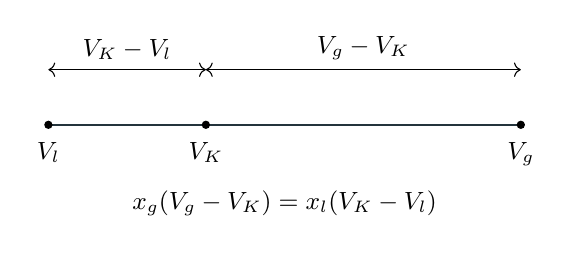
\begin{tikzpicture}[x=1cm,y=1cm,font=\small,every node/.append style={align=center}]\draw[object] (0,1)--(6,1);\foreach \x/\lab in {0/V_l,2/V_K,6/V_g}{\fill (\x,1) circle (1.5pt);\node[below] at (\x,.9){$\lab$};}
\draw[<->] (0,1.7)--(2,1.7) node[midway,above]{$V_K-V_l$};\draw[<->] (2,1.7)--(6,1.7) node[midway,above]{$V_g-V_K$};
\node at (3,0){$x_g(V_g-V_K)=x_l(V_K-V_l)$};\end{tikzpicture}\figcaption{解图 热4.3B　杠杆规则给摩尔分数，乘各相摩尔体积才得体积分数。}\end{minipage}\end{center}
\textbf{20℃装填数值。} 解图热4.3B用两相摩尔体积分配总物质的量，下面再由临界条件确定计算所需的气体常量。临界等温线在临界点有水平拐点，因此
\[
-\frac{RT_K}{(V_K-b)^2}+\frac{2a}{V_K^3}=0,\qquad
\frac{2RT_K}{(V_K-b)^3}-\frac{6a}{V_K^4}=0.
\]
分别改写为$RT_K=2a(V_K-b)^2/V_K^3$与
$RT_K=3a(V_K-b)^3/V_K^4$，相除得$2V_K=3(V_K-b)$。
故$V_K=3b$，回代第一式求$T_K$，再代状态方程求$p_K$，得到
\[
V_K=3b,\qquad p_K=\frac a{27b^2},\qquad T_K=\frac{8a}{27Rb}.
\]
因此，用SI单位$p_K=34.60\times101325\,\mathrm{Pa}$，有
\[
b=\frac{RT_K}{8p_K}=1.38427\times10^{-4}\,\mathrm{m^3/mol},\qquad
a=27p_Kb^2=1.81385\,\mathrm{Pa\cdot m^6/mol^2},
\]
\[
V_K=4.15282\times10^{-4}\,\mathrm{m^3/mol},\qquad T=293.15\,\mathrm K.
\]
按$V_g\gg V_l$近似，
\[
V_l=1.83846\times10^{-4},\qquad V_g=7.20938\times10^{-3}\quad(\mathrm{m^3/mol}),
\]
\[
B_l=\frac{(V_g-V_K)V_l}{(V_g-V_l)V_K}=0.428117,\quad
\result{B_l\simeq42.8\%,\quad B_g\simeq57.2\%\quad\text{（近似）}}.
\]
同一温度下，联立等压与等面积条件数值求解得
\[
V_l=1.83202\times10^{-4},\quad V_g=5.51626\times10^{-3}\,\mathrm{m^3/mol},
\quad p_s=3.93619\times10^5\,\mathrm{Pa},
\]
\[
\result{B_l=42.20\%,\quad B_g=57.80\%\quad\text{（完整范德瓦耳斯模型）}}.
\]
近似液相体积与完整值接近，最终液相体积比例相差约0.62个百分点。气相体积由指数式给出，对指数误差较敏感。接近临界点时 $V_g/V_l$ 趋于1，改用完整共存方程。近似要求比较 $V_g$ 与 $V_l$，而固定的 $V_K=3b$ 和液相摩尔体积 $V_l>b$ 属同一量级。
\subsubsection*{等面积条件与两相平衡的联系}
解图热4.3A的两个共存端点温度、压强和摩尔吉布斯势分别相等。
等温时$\dd g=V\dd p$，把状态方程的均匀流体支作数学延拓，分部积分得
\[
g_g-g_l=\int_{V_l}^{V_g}V\frac{\partial p}{\partial V}\dd V
=p_s(V_g-V_l)-\int_{V_l}^{V_g}p\dd V.
\]
所以两相化学势相等恰给等面积条件。
图中水平线上各点是两相按不同比例混合的状态。回环由均匀流体状态方程延拓得到，其中正斜率段的等温压缩系数为负，属于不稳定的均匀状态。
图A选$T/T_K=0.85$绘制完整状态方程，低于水平线和高于水平线的阴影面积相等。
这张图说明共存条件；20℃的具体端点仍由其自身温度求解。

还可展开上述消元的中间计算。
两端等压式相减并约去$V_g-V_l$，得
\[
RT=\frac{a(V_g+V_l)(V_g-b)(V_l-b)}{V_g^2V_l^2},\qquad
p_s=\frac{a[V_gV_l-b(V_g+V_l)]}{V_g^2V_l^2}.
\]
将第二式乘$V_g-V_l$，
\[
p_s(V_g-V_l)=a\left(\frac1{V_l}-\frac1{V_g}\right)
\left(1-\frac b{V_l}-\frac b{V_g}\right).
\]
与等面积积分式中的吸引项相加，正好得到前面完整方程组的第一个式子。
用两端同压确定同一等温线上的候选端点，再用等面积条件选出饱和压强。

\subsubsection*{液相小根的适用温度与体积误差}
为了避免低温下$a-\sqrt{a(a-4bRT)}$的相近量相减，
液相近似根也可有理化为
\[
V_l=\frac{2ab}{a+\sqrt{a(a-4bRT)}}.
\]
温度趋低时它趋近b，并仍应从大于b的一侧取值。
这个二次方程有实根的条件为
\[
T\le\frac{a}{4Rb}=\frac{27}{32}T_K.
\]
等号处二根合为 $V_l=2b$，等温斜率为零。因而近似式给出严格稳定液相根的必要条件是 $T<27T_K/32$，还要满足 $V_g\gg V_l$。解图热4.3A取 $0.85T_K$，已超过这个近似上限，图中的端点由完整两相平衡方程求出。

20℃完整解给气相摩尔分数约0.04352、液相约0.95648，
气液质量比约0.04550，而气相体积比例却约57.80\%。
解图热4.3B的较短臂$V_K-V_l$决定较少的气相物质的量，
乘上大得多的气相摩尔体积后，它仍能占过半管容积。
用给出的完整数值逐项比较，液相体积近似误差约0.35\%，
气相体积约30.7\%，液相体积比例则相差约0.62个百分点。
三个数分别以液相摩尔体积、气相摩尔体积和液相体积分数为比较对象。完整求解保留了范德瓦耳斯模型中的气相倒数体积项。要进一步比较实际乙醚的相平衡，还需使用实验数据或更精细的状态方程。


\Needspace{18\baselineskip}

\pdfbookmark[2]{第 4 题 毛细现象永动机方案的热力学破绽}{q4}

\section*{第 4 题\quad 毛细现象永动机方案的热力学破绽}

图示密闭装置与温度恒定的大气导热。A为完全润湿的毛细区域，B为实心隔挡，其外侧空间C较大；导管D内有可无摩擦移动的活塞E。活门F在一定正压差下打开、压差近零时关闭；G的开闭顺序相反。所有空白空间只含该液体蒸汽，底部及毛细区装同一液体。设计者假定毛细凹液面附近的饱和蒸汽压$p_1$与下方平液面附近的$p_2$相同，又用蒸汽的重力压差，声称能循环地从单一热源取热并全部变为活塞功。先说明这一推证的过程，再否定它并导出$p_1,p_2$的定量关系。设毛细半径$r$，升高$h$，液体与蒸汽密度为$\rho_l,\rho_v$，表面张力系数为$\sigma$；采用密度近似恒定的小高度模型。

\begin{center}\begin{minipage}{.96\linewidth}\centering
\begin{tikzpicture}[x=.85cm,y=.85cm,font=\small]
\draw[object] (0,0) rectangle (8,6);
\fill[blue!12] (0,0) rectangle (8,1.2);
\fill[blue!12] (0,1.2)--(1.8,1.2)--(1.8,3.2) .. controls (1.2,2.94) and (.6,2.94) .. (0,3.2)--cycle;
\fill[pattern=north east lines] (1.8,1.2) rectangle (4.8,3.2);
\draw[object] (1.8,1.2) rectangle (4.8,3.2);
\node[fill=white,inner sep=2pt] at (3.3,2.1){B：实心隔挡};\node at (.85,1.9){A};
\draw[traj] (0,3.2) .. controls (.6,2.94) and (1.2,2.94) .. (1.8,3.2);
\draw[object] (1.8,4)--(1.8,6) (1.8,4)--(3.6,4) (4.2,4)--(4.8,4);
\draw[object,very thick] (4.8,3.2)--(4.8,4);
\draw[object] (4.8,3.6)--(8.7,3.6);
\draw[object] (1.8,4)--(2.15,3.57);\node[left] at (1.75,3.75){F};
\draw[object] (4.2,4)--(3.85,3.62);\node[above] at (3.9,4.08){G};
\node at (2.95,3.6){D};\node[above right] at (4.8,4.03){E};
\node at (5.7,5.0){C：蒸汽空间};
\fill (.7,3.3) circle (1.3pt) node[above]{$p_1$};
\fill (5.8,3.3) circle (1.3pt) node[above]{$p_0$};
\fill (5.8,1.3) circle (1.3pt) node[above]{$p_2$};
\draw[guide] (5.4,3.2)--(7.5,3.2) (5.4,1.2)--(7.5,1.2);
\draw[<->] (7.2,1.2)--(7.2,3.2) node[midway,right]{$h$};
\draw[object] (0,0) rectangle (8,6);
\end{tikzpicture}\figcaption{图 热4.4　F连通A与活塞左腔D，G连通D与C；活塞右侧属于C。阀片位置仅示意通路。}\end{minipage}\end{center}

\Needspace{8\baselineskip}\subsection*{解答}

先按图热4.4的通路追踪设计者假设的循环：F连接A与D，G连接D与C，活塞E右面始终受到C的蒸汽压力。若$p_1=p_2$，而C中蒸汽下部压强$p_2=p_0+\rho_vgh$，便有$p_1>p_0$。于是F打开、G关闭，D中蒸汽把E向右推，输出功约为$\int(p_1-p_0)\dd V>0$。压差消失后F关闭、G打开，解图热4.4C中D经G与C相通，设计者认为等压下E可无功返回，C内部分蒸汽凝结、毛细区部分液体蒸发，使装置完全复原。循环内能变化为零，输出功便来自同一温度的大气所供热量。
\begin{center}\begin{minipage}{.97\linewidth}\centering
\begin{tikzpicture}[x=.72cm,y=.72cm,font=\small]
\foreach \dx in {0,7.4}{\begin{scope}[shift={(\dx,0)}]
\draw[object] (0,0) rectangle (5.7,2.3);
\draw[object] (1.4,0)--(1.4,.65) (1.4,1.45)--(1.4,2.3);
\draw[object] (1.4,1.45)--(2.65,1.45) (3.3,1.45)--(3.7,1.45);
\draw[object,very thick] (3.7,.65)--(3.7,1.45);\draw[object] (3.7,1.05)--(5.9,1.05);
\draw[object] (1.4,.65)--(3.7,.65);
\node at (.6,1.05){A};\node at (2.45,1.03){D};\node at (4.75,1.85){C};
\node[below] at (1.4,-.1){F};\node[above] at (3.5,1.65){G};\node[below] at (3.8,.45){E};
\end{scope}}
\draw[motion] (.9,1.05)--(2.05,1.05);\draw[very thick,warm] (2.65,1.45)--(3.3,1.45);
\draw[motion] (3.9,-.55)--(5.2,-.55) node[midway,below]{推出};
\node[above,align=center] at (2.8,2.5){F开、G闭\\假设$p_1>p_0$};
\draw[very thick,warm] (8.8,.65)--(8.8,1.45);
\draw[<->,accent,thick] (10.35,1.05)--(10.35,2.0);
\draw[motion] (12.5,-.55)--(11.2,-.55) node[midway,below]{设想等压返回};
\node[above,align=center] at (10.2,2.5){F闭、G开\\D、C等压};
\end{tikzpicture}\figcaption{解图 热4.4B、C　设计者设想的做功与复位阶段；左图所需的平衡压差实际不存在。}\end{minipage}\end{center}

解图热4.4B、C所设想的做功及复位若能循环，这相当于只从一个热源取热、把它全部转为功而不留下其他变化，违反第二定律。下面用静力和表面张力求两侧压强，说明即使活塞无摩擦，推出阶段也缺少压差。
\begin{center}\begin{minipage}{0.96\linewidth}\centering\begin{tikzpicture}[x=1cm,y=1cm,font=\small,every node/.append style={align=center}]\draw[object] (0,0)--(6,0);\node[below] at (4.7,-.1){平液面：$p_2$};
\draw[object] (.5,0)--(.5,2.4);\draw[object] (1.1,0)--(1.1,2.4);\draw[traj] (.5,2.15) .. controls (.7,1.85) and (.9,1.85) .. (1.1,2.15);
\node[left] at (.5,2.2){$p_1$};\node[right] at (1.1,1.75){$p_A$};\fill (4.7,2) circle (1.5pt) node[right]{$p_0$};
\draw[guide] (1.2,2)--(5.2,2);\draw[<->] (3.1,0)--(3.1,2) node[midway,right]{$h$};
\node at (3,-.8){$p_1-p_A=2\sigma/r$；液体梯度$\rho_lg$，蒸汽梯度$\rho_vg$};\end{tikzpicture}\figcaption{解图 热4.4A　先在两种介质中分别比较高度，再跨越凹液面。}\end{minipage}\end{center}
\textbf{按图逐层比较压强。} 沿解图热4.4A的高度线比较，在下方平液面处，液体与蒸汽压强均取$p_2$。高度$h$处，毛细液面下方液体压强为$p_A$，其上方蒸汽为$p_1$；C内同高度蒸汽压强为$p_0$。静水关系分别给
\[
p_A=p_2-\rho_lgh,\qquad p_0=p_2-\rho_vgh.
\]
凹液面处蒸汽侧压强高于液体侧，完全润湿时曲率半径为$r$，单界面的拉普拉斯关系是
\[
p_1-p_A=\frac{2\sigma}{r}.
\]
同温且连通的蒸汽在同一高度平衡，应有$p_1=p_0$。四式联立：
\[
\frac{2\sigma}{r}=(\rho_l-\rho_v)gh,
\qquad h=\frac{2\sigma}{(\rho_l-\rho_v)gr}.
\]
因此毛细凹液面上方的饱和蒸汽压与下方平液面附近的值不同：
\[
\result{p_1-p_2=-\rho_vgh
=-\frac{2\sigma\rho_v}{(\rho_l-\rho_v)r}<0}.
\]
活塞两边在同一高度的正确平衡压强其实相同，假想循环的驱动压差不再存在。

\textbf{饱和压强为何还与曲率有关。} 固定温度时，饱和压强还随液面曲率改变。凹液面的液侧压强较低，液相化学势降低，平衡蒸汽压也随之降低。可用两相化学势相等计算这一修正。令同温平液面饱和压强为$p_f$，凹液面处蒸汽压为$p_v$、液压为$p_l$，
摩尔质量仍记为$\mu$，两相摩尔吉布斯势记为$g_v,g_l$。
等温时$\dd g=V_m\dd p$；理想蒸汽有$V_{m,v}=RT/p$，不可压液体有$V_{m,l}=\mu/\rho_l$，故
\[
g_v(T,p_v)-g_v(T,p_f)=RT\ln\frac{p_v}{p_f},\qquad
g_l(T,p_l)-g_l(T,p_f)=\frac{\mu}{\rho_l}(p_l-p_f).
\]
平液面和凹液面处各自满足两相吉布斯势相等，再用$p_l=p_v-2\sigma/r$消去液压：
\[
RT\ln\frac{p_v}{p_f}=\frac{\mu}{\rho_l}
\left(p_v-p_f-\frac{2\sigma}{r}\right).
\]
小曲率修正下，$p_v-p_f\simeq p_f\ln(p_v/p_f)$；右侧这一项相对左侧的系数为
$\mu p_f/(\rho_lRT)=\rho_v/\rho_l\ll1$，可以略去。于是
\[
\ln\frac{p_{\rm concave}}{p_{\rm flat}}
\simeq-\frac{2\sigma\mu}{\rho_lRTr}.
\]
蒸汽静力平衡同时给$p(h)=p(0)\exp[-\mu gh/(RT)]$。在 $\rho_v\ll\rho_l$ 且 $\mu gh/(RT)\ll1$ 时，指数关系的首项给 $-\rho_vgh$，与前面的常密度式一致。
\subsubsection*{闭合压强回路与装置复位}
沿解图热4.4A从下方平液面出发，
先在液体中上升h，再跨越凹液面，最后在蒸汽中下降h回到同一平液面，
回到同一平液面时压强恢复为起点值，所以三段压强改变量相加为零：
\[
-\rho_lgh+\frac{2\sigma}{r}+\rho_vgh=0.
\]
三项沿回路的符号依次为负、正、正。上升和下降两段的合计是 $-(\rho_l-\rho_v)gh$。
由同高度蒸汽平衡$p_1=p_0$及$p_2-p_0=\rho_vgh$，
得到$p_1<p_2$。图B的活塞两侧在同一高度，实际相连的蒸汽压强是$p_1$与$p_0$，二者相等。$p_2$位于更低处，$p_2-p_0$是蒸汽柱重量造成的压差。

在两侧等压时，蒸汽对活塞的合力为零，所设返回段没有蒸汽驱动力。若用重物、弹簧或外力带动复位，循环要计入它们的状态变化和复位功。即使活塞与阀门均无摩擦，正功段两侧的$p_1=p_0$也给零压差。
若假设整个装置真能循环且从唯一温度T的热源吸收Q并输出同量功，
系统熵恢复，热源熵减少Q/T，整体熵变化为$-Q/T<0$。
整体熵减少违反第二定律。如果液量、界面面积或重物高度在末态改变，这些量的变化也属于过程结果，装置尚未完成循环复原。

\subsubsection*{保留蒸汽密度的一阶曲率修正}
前面的化学势方程还可在小压差下保留蒸汽密度项。
令$\delta p=p_v-p_f$，在平液面饱和压强附近线性化，得
\[
\left(\frac{RT}{p_f}-\frac{\mu}{\rho_l}\right)\delta p
=-\frac{2\sigma\mu}{\rho_lr}.
\]
使用平液面蒸汽的理想关系$\rho_v=\mu p_f/(RT)$，整理为
\[
\delta p=-\frac{2\sigma\rho_v}{(\rho_l-\rho_v)r}.
\]
它与液、汽静力及拉普拉斯关系联立的答案一致。
再令$\rho_v/\rho_l\ll1$，才退化为前述常用的凹面Kelvin近似。
这说明忽略液体摩尔体积相对于蒸汽摩尔体积的贡献，与忽略上升高度式中的蒸汽密度，是相配套的近似。
接近临界点时，以同一温度下的两相密度、表面张力和真实蒸汽性质求平衡。

若完全润湿改成接触角$\theta$，圆管静态弯月面的曲率项变为$2\sigma\cos\theta/r$，
毛细高度和相应小压差也同时乘$\cos\theta$。
从液体内部量接触角。$\theta<\pi/2$ 时，凹液面高于平液面，液面上蒸汽压较低。$\theta>\pi/2$ 时，弯月面凸起而整体低于大液面，两处蒸汽压差反号。


\Needspace{18\baselineskip}

\pdfbookmark[2]{第 5 题 毛细管中不同长度水柱的液面形状}{q5}

\section*{第 5 题\quad 毛细管中不同长度水柱的液面形状}

两端开口的竖直圆柱毛细管内径为1.0 mm，完全润湿水。管内水柱的高度分别为2.00 cm、4.00 cm和2.98 cm，求各情形下下液面是向液体内凹、向外凸，还是近似平面。取表面张力$\sigma=0.073\,\mathrm{N/m}$、水密度$\rho=10^3\,\mathrm{kg/m^3}$、$g=9.80\,\mathrm{m/s^2}$。上液面按半球处理；下液面允许接触线钉扎或端口约束，以有符号曲率半径描述。

\begin{center}\begin{minipage}{0.96\linewidth}\centering\begin{tikzpicture}[x=1cm,y=1cm,font=\small,every node/.append style={align=center}]\foreach \x/\h/\lab in {0/1.8/2.00,2.6/2.9/4.00,5.2/2.35/2.98}{
\draw[object] (\x,0)--(\x,3.3);\draw[object] (\x+.8,0)--(\x+.8,3.3);
\draw[traj] (\x,3) .. controls (\x+.25,2.7) and (\x+.55,2.7) .. (\x+.8,3);
\draw[guide] (\x,3-\h)--(\x+.8,3-\h);\node[below] at (\x+.4,-.2){$h=\lab\,\mathrm{cm}$};}
\node at (3,4){上液面为凹半球；虚线处下液面形状待求};\end{tikzpicture}\figcaption{图 热4.5　在同一符号约定下比较三个高度。}\end{minipage}\end{center}

\Needspace{8\baselineskip}\subsection*{解答}

取管半径$R_A=0.50\,\mathrm{mm}=5.0\times10^{-4}\,\mathrm m$。上端完全润湿液面近似凹半球，其内侧A点压强为
\[
p_A=p_0-\frac{2\sigma}{R_A}.
\]
下端内侧B点比A低$h$，故$p_B=p_A+\rho gh$。规定下液面曲率半径$R_B>0$表示向液体内部凹，$R_B<0$表示向外凸，平面为$1/R_B=0$。用同一约定写
\[
p_B=p_0-\frac{2\sigma}{R_B}.
\]
两式相减得
\[
\result{\frac1{R_B}=\frac1{R_A}-\frac{\rho gh}{2\sigma}}.
\]
\begin{center}\begin{minipage}{0.96\linewidth}\centering\begin{tikzpicture}[x=1cm,y=.65cm,font=\small]
\foreach \x in {0,3,6}{\draw[object] (\x,0)--(\x,4.7) (\x+1,0)--(\x+1,4.7);
\draw[traj] (\x,4.2)..controls(\x+.3,3.9) and(\x+.7,3.9)..(\x+1,4.2);
\node[left] at (\x,4.2){A};}
\draw[traj] (0,2.2)..controls(.3,2.55) and(.7,2.55)..(1,2.2);
\draw[traj] (3,1.22)--(4,1.22);
\draw[traj] (6,.2)..controls(6.3,-.15) and(6.7,-.15)..(7,.2);
\foreach \x/\y/\lab in {0/2.2/2.00,3/1.22/2.98,6/.2/4.00}{
\node[left] at (\x,\y){B};
\draw[<->] (\x+1.4,\y)--(\x+1.4,4.2) node[midway,right] {$h$};
\node[below] at (\x+.5,-.45){$h=\lab\,\mathrm{cm}$};}
\node[below] at (.5,-1.05){内凹};\node[below] at (3.5,-1.05){近似平面};\node[below] at (6.5,-1.05){外凸};
\end{tikzpicture}\figcaption{解图 热4.5A　上端压强固定；液柱越长，下端压强越高。}\end{minipage}\end{center}
解图热4.5A从左到右比较不同长度液柱：上端液面相同，液体内侧压强$p_A$不变；下端B越低，$p_B=p_A+\rho gh$越大。将图中的短柱、近临界柱和长柱依次代入同一个有符号曲率关系，便得到下端由内凹经平面变为外凸的次序。

令下液面为平面，得到临界高度
\[
h_c=\frac{2\sigma}{\rho gR_A}
=\frac{0.146}{1000\times9.80\times5.0\times10^{-4}}\,\mathrm m
=2.97959\,\mathrm{cm}.
\]
逐项代入，保持高度单位为米：
\begin{center}\begin{tabular}{ccc}\toprule $h/\mathrm{cm}$ & $1/R_B\,(\mathrm{m^{-1}})$ & 下端液面\\\midrule
2.00 & $2000-1342.47=657.53$ & 向液体内凹\\
4.00 & $2000-2684.93=-684.93$ & 向外凸\\
2.98 & $2000-2000.274\simeq0$ & 近似平面\\\bottomrule\end{tabular}\end{center}
前两种曲率半径约为$+1.52\,\mathrm{mm}$、$-1.46\,\mathrm{mm}$。第三种高度与 $h_c$ 的相对差约为 $0.014\%$，按给定精度判为近似平面。

较短水柱的下端压力仍低于大气，表面向液体内凹；较长水柱的下端压力超过大气，表面向外凸。本题让下端的接触线钉在端口或由端口提供约束，曲率便可按液柱重量所需的压差调整。
\subsubsection*{压力方向、球面近似与可支持高度}
解图热4.5A的A点取在上液面液体侧，B点取在下液面液体侧，
高度h比较这两个液内参考点。
上端压降$2\sigma/R_A=292$ Pa固定，液体向下的静水增量分别约196、392和292 Pa。
因此短柱的$p_B-p_0\simeq-96$ Pa，长柱约$+100$ Pa，临界柱接近零；
压强符号与图中下液面凹、凸、平逐一对应。
每个液面各为单个液汽界面，跨该界面的压差大小为 $2\sigma/|R|$。

球面近似还需比较弯月面尺度的重力和表面张力。
以管半径r定义$\mathrm{Bo}=\rho gr^2/\sigma$，本题约0.0336，
说明一个弯月面内部的重力压差相对曲率压差较小。
整柱压强增量为 $\rho gh$。当 $h$ 远大于管径时，该项可与上端的曲率压差同量级。
液面附近的高度定义、端口形状及接触角约束会影响更高精度的曲面解；
这里按题设的球面与柱高模型计算，第三组只作近似平面判断。

\begin{center}\begin{minipage}{.96\linewidth}\centering
\begin{tikzpicture}[x=1.25cm,y=1cm,font=\small]
\draw[axis] (0,0)--(4.8,0) node[right] {$h/\mathrm{cm}$};
\draw[axis] (0,-1.1)--(0,2.5) node[above] {$R_B^{-1}/(10^3\,\mathrm{m^{-1}})$};
\draw[traj,domain=0:4.4] plot (\x,{2-0.671232876712*\x});
\draw[guide] (2,0) node[below] {$2$}--(2,.6575342466);
\draw[guide] (4,0) node[above] {$4$}--(4,-.6849315068);
\fill (2.979591837,0) circle(1.5pt) node[above right] {$h_c\simeq2.98$};
\node[left] at (0,2) {$2$};\node at (1.5,1.7) {内凹};\node at (3.6,-1) {外凸};
\end{tikzpicture}
\figcaption{解图 热4.5B　有符号曲率随高度线性下降，零曲率对应平面。}
\end{minipage}\end{center}
解图热4.5B纵轴画曲率而非半径：通过$h_c$时曲率平滑变号，
半径的绝对值趋向无穷大，对应液面平滑趋近于平面。
圆管中跨越半径r的球面截面必须满足$|R_B|\ge r$。
在上端半径等于r的近似下，代入曲率式给形式上的范围$0\le h\le2h_c$，
最大支持高度约5.96 cm，对应下端最凸的半球。
这个上界按接触线钉扎和球冠跨越管径给出。实际端口的接触角范围、脱钉或滴落条件决定可维持的最大高度。若柱长和管径接近，两端形状要一起求解。


\Needspace{18\baselineskip}

\pdfbookmark[2]{第 6 题 双液体U形毛细管表面张力比}{q6}

\section*{第 6 题\quad 双液体U形毛细管表面张力比}

总长$L$、内半径$R$均匀的倒U形毛细管，其两开口竖直向下，略浸入两种液体的等高液面。两液体密度$\rho_1,\rho_2$，与管壁接触角均为零；毛细管中气体不漏出，压缩过程等温，液体上升高度分别为$h_1,h_2$。插入前气体压强为大气压$p_0$，开口浸入深度忽略。求两液体表面张力系数$\sigma_1/\sigma_2$，并说明$h_1+h_2<L$的意义。

\begin{center}\begin{minipage}{0.96\linewidth}\centering\begin{tikzpicture}[x=1cm,y=1cm,font=\small,every node/.append style={align=center}]\fill[blue!15] (-.5,-.7) rectangle (1.8,.8);\fill[brown!15] (3.2,-.7) rectangle (5.5,.8);
\draw[object] (-.5,.8)--(1.8,.8);\draw[object] (3.2,.8)--(5.5,.8);
\draw[object] (.5,0)--(.5,3) .. controls (.5,3.5) and (4.5,3.5) ..(4.5,3)--(4.5,0);
\draw[object] (.8,0)--(.8,2.8) ..controls(.8,3.15) and(4.2,3.15)..(4.2,2.8)--(4.2,0);
\draw[traj] (.5,2.1)..controls(.6,1.95) and(.7,1.95)..(.8,2.1);
\draw[traj] (4.2,1.8)..controls(4.3,1.65) and(4.4,1.65)..(4.5,1.8);
\draw[<->] (1.3,.8)--(1.3,2.1) node[midway,right]{$h_1$};\draw[<->] (3.7,.8)--(3.7,1.8) node[midway,left]{$h_2$};
\node at (2.5,3.8){封闭气体$p$，长度$L-h_1-h_2$};\node at (.3,-.45){液体1};\node at (4.6,-.45){液体2};\end{tikzpicture}\figcaption{图 热4.6　倒U形管中的气体被两液柱共同压缩。}\end{minipage}\end{center}

\Needspace{8\baselineskip}\subsection*{解答}

沿图热4.6的倒 U 形管，管道截面积恒定，两端液柱升起使气柱长度由 $L$ 减为 $L-h_1-h_2$。封闭气体取等温理想气体，管内两端的气体静压差约为 $\rho_{\rm gas}g|h_1-h_2|$，这里忽略这项，取共同气压 $p$，得到
\[
p(L-h_1-h_2)=p_0L,
\quad p=\frac{p_0L}{L-h_1-h_2},
\quad \Delta p=p-p_0=\frac{p_0(h_1+h_2)}{L-h_1-h_2}.
\]
在液体1内，毛细液面下方的压力也可由外界等高液面计算：
\[
p_{l1}=p_0-\rho_1gh_1.
\]
完全润湿的凹半球跨面压力关系为$p-p_{l1}=2\sigma_1/R$。液体2同理。因此
\[
\frac{2\sigma_1}{R}=\Delta p+\rho_1gh_1,\qquad
\frac{2\sigma_2}{R}=\Delta p+\rho_2gh_2.
\]
\begin{center}\begin{minipage}{0.96\linewidth}\centering\begin{tikzpicture}[x=1cm,y=1cm,font=\small,every node/.append style={align=center}]\node[draw] at (2.8,2.5){$p(L-h_1-h_2)=p_0L$};
\draw[object] (0,0)--(0,1.8);\draw[object] (.7,0)--(.7,1.8);\draw[traj] (0,1.5)..controls(.2,1.2) and(.5,1.2)..(.7,1.5);
\node[left] at (0,1.6){气体$p$};\node[right] at (.7,1){$p_{l1}=p_0-\rho_1gh_1$};
\node at (3.1,.1){$2\sigma_1/R=(p-p_0)+\rho_1gh_1$\\$2\sigma_2/R=(p-p_0)+\rho_2gh_2$};\end{tikzpicture}\figcaption{解图 热4.6A　两端共用同一压强增量，而静水项各自计算。}\end{minipage}\end{center}
解图热4.6A中，对任一支液体从槽外水平面走到管内气体，压力变化可按同一路径逐段相加：
\begin{center}\begin{minipage}{0.96\linewidth}\centering
\begin{tikzpicture}[x=1cm,y=1cm]
\node[draw,minimum width=1cm] (A) at (0,0) {$p_0$};
\node[draw,minimum width=1.2cm] (B) at (3.5,0) {$p_{li}$};
\node[draw,minimum width=1cm] (C) at (7,0) {$p$};
\draw[->,thick,color=accent] (A)--(B) node[midway,above] {$-\rho_i gh_i$};
\draw[->,thick,color=accent] (B)--(C) node[midway,above] {$+2\sigma_i/R$};
\node[below] at (1.7,-.15) {沿液体向上};\node[below] at (5.25,-.15) {跨凹液面};
\end{tikzpicture}
\figcaption{解图热4.6B\quad 两支液体各有自己的静水项，但终点为同一封闭气体压强。}
\end{minipage}\end{center}
沿解图热4.6B相加得$p=p_0-\rho_i gh_i+2\sigma_i/R$。因此毛细压差要承担气体增压和液柱重力两项，所以 $p-p_{li}=\Delta p+\rho_i gh_i$。

相除消去共同管半径，并代入封闭气体的增压项，得到
\[
\result{\frac{\sigma_1}{\sigma_2}
=\frac{p_0(h_1+h_2)+\rho_1gh_1(L-h_1-h_2)}
{p_0(h_1+h_2)+\rho_2gh_2(L-h_1-h_2)}}.
\]
气体若与大气连通，取 $p=p_0$，张力比为 $\rho_1h_1/(\rho_2h_2)$。题设给出的是两支通过同一个封闭气体耦合的平衡。

\textbf{封闭气柱长度与张力比的极限。} 等温压缩关系适用于封闭气柱仍有正长度的状态，即$h_1+h_2<L$。若$h_1=h_2$且$\rho_1=\rho_2$，两边静水项相等，张力比为1。固定两液柱高度比较时，增压项远大于两个静水项，张力比趋近1。改变$L$时，则由完整平衡方程联立求新的$h_1,h_2$。
\subsubsection*{共同增压对张力差和张力比的影响}
解图热4.6B的两条路径都从槽外$p_0$出发，以同一封闭气体p结束，
但两段液体的静水压降分别为$\rho_1gh_1$和$\rho_2gh_2$。
共同的$\Delta p$是两条毛细压差中的加数，只有相减才会消去：
\[
\frac{2(\sigma_1-\sigma_2)}R
=g(\rho_1h_1-\rho_2h_2).
\]
两种张力相等时，密度和高度的乘积相等。高度之比为两种密度的反比。
在张力比中，两侧毛细压差均含共同的加数 $\Delta p$。

令$H=h_1+h_2$、$\lambda=H/L$及$G_i=\rho_igh_i/p_0$，
答案可整理为
\[
\frac{\sigma_1}{\sigma_2}
=\frac{\lambda+(1-\lambda)G_1}
{\lambda+(1-\lambda)G_2},\qquad0<\lambda<1.
\]
这个表达式分开表示封闭气体压缩和两侧重力贡献。
开孔后的公式相当于气体增压为零，
要把闭气结果近似成开孔结果，须有$\Delta p\ll\rho_igh_i$对相关两侧都成立，
即使 $H/L$ 较小，也要比较这一压缩量与两侧静水项的实际量级。

\subsubsection*{剩余气体体积与有限张力的约束}
题图给定的是管长和测得高度，气体体积按统一截面积乘剩余长度计算。
这里忽略弯月面的端部体积和极小浸入深度，管子弯曲部分的长度已计入总长L。
若端部体积不可忽略，应直接用实际气体体积写$pV_g=p_0V_{g0}$，
实际气体体积包括弯管部分。两侧静水压仍按各自界面与槽面的竖直高度差计算。

由于两液体都上升，$\rho_igh_i>0$，有限的毛细压差要求
\[
\Delta p<\min\left(\frac{2\sigma_1}R,\frac{2\sigma_2}R\right)=c,
\qquad H<\frac{c}{p_0+c}L<L.
\]
每侧还有$h_i<2\sigma_i/(\rho_i gR)$。
有限表面张力给 $H<[c/(p_0+c)]L$，可达的上升总长早于气柱体积趋零。改变管长、排气状态或温度时，新的高度由气体和两支液柱的方程联立确定。


\Needspace{18\baselineskip}

\pdfbookmark[2]{第 7 题 微小水滴的曲率压强与密度变化}{q7}

\section*{第 7 题\quad 微小水滴的曲率压强与密度变化}

4℃、1 atm时水的表面张力$\sigma=7.24\times10^{-2}\,\mathrm{N/m}$，等温压缩系数$\beta=-(1/V)(\partial V/\partial p)_T=4.75\times10^{-5}\,\mathrm{atm^{-1}}$。同温、同外压下，平液面附近水的密度为$\rho_0$。求半径$r=1.0\times10^{-6}\,\mathrm{cm}$的微小水滴密度。计算中取$\sigma,\beta$为常量，并讨论该连续介质估算的条件。

\begin{center}\begin{minipage}{0.96\linewidth}\centering\begin{tikzpicture}[x=1cm,y=1cm,font=\small,every node/.append style={align=center}]\fill[blue!12] (0,0) circle (1.2);\draw[object] (0,0) circle (1.2);\draw[guide] (0,0)--(1.2,0) node[midway,above]{$r$};
\node at (0,-.45){$p,\rho$};\node at (2.2,1.2){外压$p_0$};\draw[force] (1.2,0)--(.84,0);
\draw[force] (-1.2,0)--(-.84,0);\node at (3,-.5){$p-p_0=2\sigma/r$};
\node[below] at (0,-1.22){箭头为张力在小曲面上的合力};\end{tikzpicture}\figcaption{图 热4.7　球形水滴只有一个界面，外压不是滴内压强。}\end{minipage}\end{center}

\Needspace{8\baselineskip}\subsection*{解答}

图中液滴为单界面球面，滴内压强高于外压：$p-p_0=2\sigma/r$。压缩系数描述同一份水随压力的体积变化。在等温、$\beta$取常量时，
\[
\beta\dd p=-\frac{\dd V}{V},\qquad
\beta(p-p_0)=\ln\frac{V_0}{V}.
\]
同质量下$\rho V=\rho_0V_0$，于是
\[
\ln\frac{\rho}{\rho_0}=\beta(p-p_0),\qquad
\result{\rho=\rho_0\exp\left(\frac{2\sigma\beta}{r}\right)}.
\]
\begin{center}\begin{minipage}{0.96\linewidth}\centering\begin{tikzpicture}[x=4.7cm,y=1.35cm,font=\small]
\draw[axis] (0,0)--(1.2,0) node[right] {$z=2\sigma\beta/r$};
\draw[axis] (0,0)--(0,3.1) node[above] {$\rho/\rho_0$};
\draw[traj,domain=0:1,samples=100] plot(\x,{exp(\x)});
\draw[warm,thick,dashed,domain=0:1] plot(\x,{1+\x});
\foreach \x in {.5,1}{\draw (\x,-.04)--(\x,.04) node[below=3pt] {$\x$};}
\foreach \y in {1,2}{\draw (-.015,\y)--(.015,\y) node[left=3pt] {$\y$};}
\node[right] at (.82,2.7) {$e^z$};\node[right] at (.88,1.75) {$1+z$};
\end{tikzpicture}\figcaption{解图 热4.7A　先积分压缩系数，再用小指数作近似。}\end{minipage}\end{center}
指数关系使用的是同质量水的体积变化，而$r$是最终液滴的曲率半径。由质量守恒，
\[\frac{V}{V_0}=\frac{\rho_0}{\rho}=e^{-z},\qquad
\frac{r_0}{r}=\left(\frac{V_0}{V}\right)^{1/3}=e^{z/3},\quad
z=\frac{2\sigma\beta}{r}.\]
其中 $r_0$ 表示同质量水在外压 $p_0$ 下的参考半径。拉普拉斯压差按实际液面的曲率半径 $r$ 计算。题图热4.7的箭头表示液面小面元所受张力的向内合力。张力沿小面元的边缘作切向牵引，曲率使这些牵引有向内的合量；内外压差提供向外的平衡力。内压升高使同质量的水体积减小、密度增大，即 $V<V_0$、$\rho>\rho_0$。

数值计算先统一单位：
\[
r=1.0\times10^{-6}\,\mathrm{cm}=1.0\times10^{-8}\,\mathrm m,
\quad \beta=\frac{4.75\times10^{-5}}{101325}\,\mathrm{Pa^{-1}}
=4.68789\times10^{-10}\,\mathrm{Pa^{-1}}.
\]
曲率压差及无量纲指数为
\[
\Delta p=\frac{0.1448}{10^{-8}}=1.448\times10^7\,\mathrm{Pa},
\quad z=\beta\Delta p=6.78806\times10^{-3}.
\]
所以
\[
\frac{\rho}{\rho_0}=e^z=1.006811,
\quad \rho\simeq\rho_0(1+z)=1.006788\rho_0\simeq1.0068\rho_0.
\]
密度约增加0.68\%。曲率压差约143 atm，仍只造成小相对密度变化，原因是水的压缩系数很小。把指数保留到一次项，相对于总密度的误差约为 $z^2/2=2.3\times10^{-5}$。这里把 $10\,\mathrm{nm}$ 液滴视为连续液体，并在所用压差内取常量 $\beta$ 和 $\sigma$。
\subsubsection*{半球受力、压缩量与线性近似}
将题图热4.7中的液滴沿过球心平面剖成两半，
内外压力差在圆截面上的合力为$\Delta p\,\pi r^2$，
球面张力沿周长$2\pi r$的合力为$2\pi r\sigma$。
平衡给$\Delta p=2\sigma/r$，方向指向滴外的内压与收缩液面的表面张力相抵。
半球圆周和截面都由同一个实际半径决定，所以周长除以面积正比于 $1/r$。

在积分中，$\dd V/V=-\dd\rho/\rho$来自质量不变，
因此压缩系数也可写成$\beta=(1/\rho)(\partial\rho/\partial p)_T$。
积分从外压$p_0$起，到滴内压$p_0+2\sigma/r$止。压强升高使密度增加，固定质量的体积相应减小。
本题数值还给$V/V_0\simeq0.993235$及$r_0/r\simeq1.002265$，
体积缩小约 $0.677\%$。由 $r/r_0=e^{-z/3}$ 得半径缩小约 $0.226\%$，约为体积相对变化量的三分之一。

解图热4.7A同时画$e^z$与$1+z$，两曲线在$z=0$相切，
正指数时指数曲线始终在切线上方，所以一阶式略低估密度。
本题$z\simeq0.006788$，两式差为密度基准的约$2.31\times10^{-5}$，
相对于精确密度的误差约$2.29\times10^{-5}$；
若所求量是密度增量，以 $e^z-1$ 作分母，得到的相对误差约为 $z/2=0.34\%$。
两个相对误差的分母分别是精确总密度和密度增加量，后者较小，因此相对误差较大。
如果题目改为给定同质量在外压下的半径$r_0$，
则用质量关系$\rho/\rho_0=(r_0/r)^3$与曲率压差联立求实际半径$r$，再代入密度指数式。


\Needspace{18\baselineskip}

\pdfbookmark[2]{第 8 题 相通肥皂泡的稳定与不稳定平衡}{q8}

\section*{第 8 题\quad 相通肥皂泡的稳定与不稳定平衡}

两相同球冠形肥皂泡A、B固定在半径$r_1$相同的圆管口上；外界压强相同，两泡连通，外部供气阀K关闭，连接泡的阀门保持开启。表面张力系数恒定，忽略液膜厚度和气体密度变化。证明：两泡均小于半球时等形平衡稳定，均大于半球时等形平衡不稳定。后一情形取$r_1=2.00\,\mathrm{cm}$、初始球面曲率半径$r_2=2.50\,\mathrm{cm}$，求一泡变小、另一泡变大后再次平衡的曲率半径与球冠高度。

\begin{center}\begin{minipage}{0.96\linewidth}\centering\begin{tikzpicture}[x=1cm,y=1cm,font=\small,every node/.append style={align=center}]\draw[traj] (-0.7500,0.0000) -- (-0.7389,0.0201) -- (-0.7273,0.0399) -- (-0.7151,0.0594) -- (-0.7025,0.0786) -- (-0.6893,0.0974) -- (-0.6756,0.1158) -- (-0.6614,0.1339) -- (-0.6467,0.1516) -- (-0.6316,0.1688) -- (-0.6160,0.1857) -- (-0.6000,0.2021) -- (-0.5835,0.2181) -- (-0.5666,0.2336) -- (-0.5492,0.2487) -- (-0.5315,0.2633) -- (-0.5134,0.2774) -- (-0.4949,0.2911) -- (-0.4761,0.3042) -- (-0.4569,0.3168) -- (-0.4373,0.3289) -- (-0.4175,0.3404) -- (-0.3973,0.3514) -- (-0.3769,0.3619) -- (-0.3561,0.3718) -- (-0.3352,0.3811) -- (-0.3139,0.3899) -- (-0.2925,0.3981) -- (-0.2708,0.4057) -- (-0.2489,0.4127) -- (-0.2269,0.4192) -- (-0.2047,0.4250) -- (-0.1823,0.4302) -- (-0.1598,0.4348) -- (-0.1372,0.4389) -- (-0.1145,0.4423) -- (-0.0917,0.4450) -- (-0.0688,0.4472) -- (-0.0459,0.4488) -- (-0.0230,0.4497) -- (0.0000,0.4500) -- (0.0230,0.4497) -- (0.0459,0.4488) -- (0.0688,0.4472) -- (0.0917,0.4450) -- (0.1145,0.4423) -- (0.1372,0.4389) -- (0.1598,0.4348) -- (0.1823,0.4302) -- (0.2047,0.4250) -- (0.2269,0.4192) -- (0.2489,0.4127) -- (0.2708,0.4057) -- (0.2925,0.3981) -- (0.3139,0.3899) -- (0.3352,0.3811) -- (0.3561,0.3718) -- (0.3769,0.3619) -- (0.3973,0.3514) -- (0.4175,0.3404) -- (0.4373,0.3289) -- (0.4569,0.3168) -- (0.4761,0.3042) -- (0.4949,0.2911) -- (0.5134,0.2774) -- (0.5315,0.2633) -- (0.5492,0.2487) -- (0.5666,0.2336) -- (0.5835,0.2181) -- (0.6000,0.2021) -- (0.6160,0.1857) -- (0.6316,0.1688) -- (0.6467,0.1516) -- (0.6614,0.1339) -- (0.6756,0.1158) -- (0.6893,0.0974) -- (0.7025,0.0786) -- (0.7151,0.0594) -- (0.7273,0.0399) -- (0.7389,0.0201) -- (0.7500,0.0000);\draw[object] (-0.75,0)--(-.2,0) (.2,0)--(.75,0);\draw[traj] (2.2500,0.0000) -- (2.2611,0.0201) -- (2.2727,0.0399) -- (2.2849,0.0594) -- (2.2975,0.0786) -- (2.3107,0.0974) -- (2.3244,0.1158) -- (2.3386,0.1339) -- (2.3533,0.1516) -- (2.3684,0.1688) -- (2.3840,0.1857) -- (2.4000,0.2021) -- (2.4165,0.2181) -- (2.4334,0.2336) -- (2.4508,0.2487) -- (2.4685,0.2633) -- (2.4866,0.2774) -- (2.5051,0.2911) -- (2.5239,0.3042) -- (2.5431,0.3168) -- (2.5627,0.3289) -- (2.5825,0.3404) -- (2.6027,0.3514) -- (2.6231,0.3619) -- (2.6439,0.3718) -- (2.6648,0.3811) -- (2.6861,0.3899) -- (2.7075,0.3981) -- (2.7292,0.4057) -- (2.7511,0.4127) -- (2.7731,0.4192) -- (2.7953,0.4250) -- (2.8177,0.4302) -- (2.8402,0.4348) -- (2.8628,0.4389) -- (2.8855,0.4423) -- (2.9083,0.4450) -- (2.9312,0.4472) -- (2.9541,0.4488) -- (2.9770,0.4497) -- (3.0000,0.4500) -- (3.0230,0.4497) -- (3.0459,0.4488) -- (3.0688,0.4472) -- (3.0917,0.4450) -- (3.1145,0.4423) -- (3.1372,0.4389) -- (3.1598,0.4348) -- (3.1823,0.4302) -- (3.2047,0.4250) -- (3.2269,0.4192) -- (3.2489,0.4127) -- (3.2708,0.4057) -- (3.2925,0.3981) -- (3.3139,0.3899) -- (3.3352,0.3811) -- (3.3561,0.3718) -- (3.3769,0.3619) -- (3.3973,0.3514) -- (3.4175,0.3404) -- (3.4373,0.3289) -- (3.4569,0.3168) -- (3.4761,0.3042) -- (3.4949,0.2911) -- (3.5134,0.2774) -- (3.5315,0.2633) -- (3.5492,0.2487) -- (3.5666,0.2336) -- (3.5835,0.2181) -- (3.6000,0.2021) -- (3.6160,0.1857) -- (3.6316,0.1688) -- (3.6467,0.1516) -- (3.6614,0.1339) -- (3.6756,0.1158) -- (3.6893,0.0974) -- (3.7025,0.0786) -- (3.7151,0.0594) -- (3.7273,0.0399) -- (3.7389,0.0201) -- (3.7500,0.0000);\draw[object] (2.25,0)--(2.8,0) (3.2,0)--(3.75,0);\draw[traj] (-0.7500,-3.0000) -- (-0.7800,-2.9576) -- (-0.8076,-2.9137) -- (-0.8327,-2.8683) -- (-0.8552,-2.8215) -- (-0.8752,-2.7736) -- (-0.8924,-2.7247) -- (-0.9069,-2.6749) -- (-0.9187,-2.6243) -- (-0.9276,-2.5732) -- (-0.9337,-2.5217) -- (-0.9369,-2.4699) -- (-0.9373,-2.4180) -- (-0.9348,-2.3662) -- (-0.9294,-2.3146) -- (-0.9212,-2.2633) -- (-0.9101,-2.2126) -- (-0.8963,-2.1626) -- (-0.8797,-2.1135) -- (-0.8604,-2.0653) -- (-0.8385,-2.0182) -- (-0.8140,-1.9725) -- (-0.7871,-1.9282) -- (-0.7577,-1.8854) -- (-0.7260,-1.8443) -- (-0.6920,-1.8051) -- (-0.6560,-1.7677) -- (-0.6179,-1.7325) -- (-0.5780,-1.6994) -- (-0.5362,-1.6685) -- (-0.4929,-1.6400) -- (-0.4480,-1.6140) -- (-0.4017,-1.5904) -- (-0.3543,-1.5695) -- (-0.3057,-1.5512) -- (-0.2562,-1.5357) -- (-0.2059,-1.5229) -- (-0.1550,-1.5129) -- (-0.1036,-1.5057) -- (-0.0519,-1.5014) -- (0.0000,-1.5000) -- (0.0519,-1.5014) -- (0.1036,-1.5057) -- (0.1550,-1.5129) -- (0.2059,-1.5229) -- (0.2562,-1.5357) -- (0.3057,-1.5512) -- (0.3543,-1.5695) -- (0.4017,-1.5904) -- (0.4480,-1.6140) -- (0.4929,-1.6400) -- (0.5362,-1.6685) -- (0.5780,-1.6994) -- (0.6179,-1.7325) -- (0.6560,-1.7677) -- (0.6920,-1.8051) -- (0.7260,-1.8443) -- (0.7577,-1.8854) -- (0.7871,-1.9282) -- (0.8140,-1.9725) -- (0.8385,-2.0182) -- (0.8604,-2.0653) -- (0.8797,-2.1135) -- (0.8963,-2.1626) -- (0.9101,-2.2126) -- (0.9212,-2.2633) -- (0.9294,-2.3146) -- (0.9348,-2.3662) -- (0.9373,-2.4180) -- (0.9369,-2.4699) -- (0.9337,-2.5217) -- (0.9276,-2.5732) -- (0.9187,-2.6243) -- (0.9069,-2.6749) -- (0.8924,-2.7247) -- (0.8752,-2.7736) -- (0.8552,-2.8215) -- (0.8327,-2.8683) -- (0.8076,-2.9137) -- (0.7800,-2.9576) -- (0.7500,-3.0000);\draw[object] (-0.75,-3)--(-.2,-3) (.2,-3)--(.75,-3);\draw[traj] (2.2500,-3.0000) -- (2.2200,-2.9576) -- (2.1924,-2.9137) -- (2.1673,-2.8683) -- (2.1448,-2.8215) -- (2.1248,-2.7736) -- (2.1076,-2.7247) -- (2.0931,-2.6749) -- (2.0813,-2.6243) -- (2.0724,-2.5732) -- (2.0663,-2.5217) -- (2.0631,-2.4699) -- (2.0627,-2.4180) -- (2.0652,-2.3662) -- (2.0706,-2.3146) -- (2.0788,-2.2633) -- (2.0899,-2.2126) -- (2.1037,-2.1626) -- (2.1203,-2.1135) -- (2.1396,-2.0653) -- (2.1615,-2.0182) -- (2.1860,-1.9725) -- (2.2129,-1.9282) -- (2.2423,-1.8854) -- (2.2740,-1.8443) -- (2.3080,-1.8051) -- (2.3440,-1.7677) -- (2.3821,-1.7325) -- (2.4220,-1.6994) -- (2.4638,-1.6685) -- (2.5071,-1.6400) -- (2.5520,-1.6140) -- (2.5983,-1.5904) -- (2.6457,-1.5695) -- (2.6943,-1.5512) -- (2.7438,-1.5357) -- (2.7941,-1.5229) -- (2.8450,-1.5129) -- (2.8964,-1.5057) -- (2.9481,-1.5014) -- (3.0000,-1.5000) -- (3.0519,-1.5014) -- (3.1036,-1.5057) -- (3.1550,-1.5129) -- (3.2059,-1.5229) -- (3.2562,-1.5357) -- (3.3057,-1.5512) -- (3.3543,-1.5695) -- (3.4017,-1.5904) -- (3.4480,-1.6140) -- (3.4929,-1.6400) -- (3.5362,-1.6685) -- (3.5780,-1.6994) -- (3.6179,-1.7325) -- (3.6560,-1.7677) -- (3.6920,-1.8051) -- (3.7260,-1.8443) -- (3.7577,-1.8854) -- (3.7871,-1.9282) -- (3.8140,-1.9725) -- (3.8385,-2.0182) -- (3.8604,-2.0653) -- (3.8797,-2.1135) -- (3.8963,-2.1626) -- (3.9101,-2.2126) -- (3.9212,-2.2633) -- (3.9294,-2.3146) -- (3.9348,-2.3662) -- (3.9373,-2.4180) -- (3.9369,-2.4699) -- (3.9337,-2.5217) -- (3.9276,-2.5732) -- (3.9187,-2.6243) -- (3.9069,-2.6749) -- (3.8924,-2.7247) -- (3.8752,-2.7736) -- (3.8552,-2.8215) -- (3.8327,-2.8683) -- (3.8076,-2.9137) -- (3.7800,-2.9576) -- (3.7500,-3.0000);\draw[object] (2.25,-3)--(2.8,-3) (3.2,-3)--(3.75,-3);
\draw[object] (-.2,0)--(-.2,-.62)--(3.2,-.62)--(3.2,0) (.2,0)--(.2,-.30)--(2.8,-.30)--(2.8,0);
\draw[object] (-.2,-3)--(-.2,-3.62)--(3.2,-3.62)--(3.2,-3) (.2,-3)--(.2,-3.30)--(2.8,-3.30)--(2.8,-3);
\node at (1.5,1.2){小于半球};\node at (1.5,-.9){两泡连通};\node at (1.5,-3.9){大于半球};\end{tikzpicture}\figcaption{图 热4.8　同一管口的球冠越高，曲率半径未必越大。}\end{minipage}\end{center}

\Needspace{8\baselineskip}\subsection*{解答}

取固定管口半径$a=r_1$，球冠高度为$h$，曲率半径为$R_c$。轴截面的直角三角形给
\[
a^2+(R_c-h)^2=R_c^2,
\quad R_c=\frac{a^2+h^2}{2h}.
\]
肥皂膜有两个界面，故内外压差及球冠体积为
\[
\Delta p(h)=\frac{4\sigma}{R_c}=\frac{8\sigma h}{a^2+h^2},
\quad V(h)=\frac{\pi h}{6}(3a^2+h^2).
\]
其导数分别为
\[
\frac{\dd\Delta p}{\dd h}=\frac{8\sigma(a^2-h^2)}{(a^2+h^2)^2},
\qquad\frac{\dd V}{\dd h}=\frac\pi2(a^2+h^2)>0.
\]
\begin{center}\begin{minipage}{0.96\linewidth}\centering\begin{tikzpicture}[x=1.7cm,y=2.4cm,font=\small]
\draw[axis] (0,0)--(3.65,0) node[right] {$u=h/a$};
\draw[axis] (0,0)--(0,1.45) node[above] {$\Delta p/(4\sigma/a)$};
\draw[traj,domain=0:3.4,samples=130] plot(\x,{2*\x/(1+\x*\x)});
\draw[guide] (1,0) node[below] {$1$}--(1,1)--(0,1) node[left] {$1$};
\draw[warm,dashed] (.375833,0.658632)--(2.660754,0.658632);
\fill (.375833,.658632) circle(1.4pt);\fill (2.660754,.658632) circle(1.4pt);
\node[above left] at (.85,1.12) {同形稳定支};\node[above] at (2.45,1.12) {同形不稳定支};
\node[below] at (2.4,.46) {虚线连接一小一大新平衡};
\end{tikzpicture}\figcaption{解图 热4.8A　压强对球冠高度先升后降，半球处达到最大。}\end{minipage}\end{center}
\textbf{同形平衡的稳定性。} 对照解图热4.8A的压强曲线，当$h<a$，两泡均小于半球，增加体积会增加压强。若A略缩小，A压强下降，气体从B流回A，体积差随回流减小，平衡稳定。若$h>a$，增加体积反而降低压强。A略缩小时压强升高，气体由A流向B；A更小、B更大，扰动被放大，平衡不稳定。固定管口时，曲率半径按 $R_c=(a^2+h^2)/(2h)$ 变化，浅冠和大冠的 $\dd p/\dd V$ 分别为正和负。恰在$h=a$时一阶导数为零，需用更高阶项判定。

\textbf{再次平衡的几何与守恒。} 气体密度变化忽略，总泡体积守恒。初始两泡都是大球冠，故
\[
h_0=r_2+\sqrt{r_2^2-r_1^2}=2.50+\sqrt{6.25-4.00}=4.00\,\mathrm{cm}.
\]
每泡体积
\[
V_0=\pi h_0^2\left(r_2-\frac{h_0}{3}\right)
=\pi\times16\left(2.50-\frac43\right)
=\frac{56\pi}{3}\,\mathrm{cm^3}.
\]
新平衡两泡压强相等，因外压、$\sigma$相同，它们的曲率半径同为$r$。一泡是小球冠，另一泡是大球冠，管口相同，它们恰是一个球的互补两部分：
\[
h_-=r-\sqrt{r^2-r_1^2},\qquad h_+=r+\sqrt{r^2-r_1^2},
\quad V(h_-)+V(h_+)=\frac{4\pi r^3}{3}.
\]
\begin{center}\begin{minipage}{0.96\linewidth}\centering\begin{tikzpicture}[x=1cm,y=1cm,font=\small,every node/.append style={align=center}]\draw[traj] (-1.0000,0.0000) -- (-0.9793,0.0178) -- (-0.9583,0.0352) -- (-0.9370,0.0522) -- (-0.9153,0.0689) -- (-0.8934,0.0851) -- (-0.8712,0.1010) -- (-0.8487,0.1165) -- (-0.8260,0.1315) -- (-0.8029,0.1461) -- (-0.7796,0.1604) -- (-0.7561,0.1742) -- (-0.7323,0.1875) -- (-0.7083,0.2005) -- (-0.6840,0.2130) -- (-0.6595,0.2251) -- (-0.6349,0.2367) -- (-0.6100,0.2479) -- (-0.5849,0.2586) -- (-0.5596,0.2689) -- (-0.5341,0.2787) -- (-0.5085,0.2881) -- (-0.4827,0.2970) -- (-0.4568,0.3055) -- (-0.4307,0.3134) -- (-0.4044,0.3210) -- (-0.3781,0.3280) -- (-0.3516,0.3345) -- (-0.3250,0.3406) -- (-0.2982,0.3462) -- (-0.2714,0.3513) -- (-0.2445,0.3560) -- (-0.2176,0.3601) -- (-0.1905,0.3638) -- (-0.1634,0.3670) -- (-0.1363,0.3697) -- (-0.1091,0.3719) -- (-0.0818,0.3736) -- (-0.0546,0.3748) -- (-0.0273,0.3756) -- (0.0000,0.3758) -- (0.0273,0.3756) -- (0.0546,0.3748) -- (0.0818,0.3736) -- (0.1091,0.3719) -- (0.1363,0.3697) -- (0.1634,0.3670) -- (0.1905,0.3638) -- (0.2176,0.3601) -- (0.2445,0.3560) -- (0.2714,0.3513) -- (0.2982,0.3462) -- (0.3250,0.3406) -- (0.3516,0.3345) -- (0.3781,0.3280) -- (0.4044,0.3210) -- (0.4307,0.3134) -- (0.4568,0.3055) -- (0.4827,0.2970) -- (0.5085,0.2881) -- (0.5341,0.2787) -- (0.5596,0.2689) -- (0.5849,0.2586) -- (0.6100,0.2479) -- (0.6349,0.2367) -- (0.6595,0.2251) -- (0.6840,0.2130) -- (0.7083,0.2005) -- (0.7323,0.1875) -- (0.7561,0.1742) -- (0.7796,0.1604) -- (0.8029,0.1461) -- (0.8260,0.1315) -- (0.8487,0.1165) -- (0.8712,0.1010) -- (0.8934,0.0851) -- (0.9153,0.0689) -- (0.9370,0.0522) -- (0.9583,0.0352) -- (0.9793,0.0178) -- (1.0000,0.0000);\draw[object] (-1,0)--(1,0);\draw[traj] (3.0000,0.0000) -- (2.9327,0.0626) -- (2.8693,0.1292) -- (2.8100,0.1995) -- (2.7551,0.2733) -- (2.7048,0.3502) -- (2.6592,0.4301) -- (2.6185,0.5125) -- (2.5829,0.5973) -- (2.5525,0.6841) -- (2.5275,0.7725) -- (2.5078,0.8623) -- (2.4935,0.9532) -- (2.4848,1.0447) -- (2.4817,1.1366) -- (2.4841,1.2285) -- (2.4921,1.3201) -- (2.5056,1.4110) -- (2.5246,1.5010) -- (2.5490,1.5896) -- (2.5787,1.6766) -- (2.6137,1.7617) -- (2.6537,1.8445) -- (2.6987,1.9247) -- (2.7484,2.0020) -- (2.8027,2.0762) -- (2.8614,2.1469) -- (2.9243,2.2140) -- (2.9911,2.2771) -- (3.0617,2.3361) -- (3.1356,2.3907) -- (3.2128,2.4408) -- (3.2928,2.4860) -- (3.3754,2.5264) -- (3.4603,2.5616) -- (3.5472,2.5917) -- (3.6358,2.6165) -- (3.7256,2.6358) -- (3.8165,2.6497) -- (3.9081,2.6580) -- (4.0000,2.6608) -- (4.0919,2.6580) -- (4.1835,2.6497) -- (4.2744,2.6358) -- (4.3642,2.6165) -- (4.4528,2.5917) -- (4.5397,2.5616) -- (4.6246,2.5264) -- (4.7072,2.4860) -- (4.7872,2.4408) -- (4.8644,2.3907) -- (4.9383,2.3361) -- (5.0089,2.2771) -- (5.0757,2.2140) -- (5.1386,2.1469) -- (5.1973,2.0762) -- (5.2516,2.0020) -- (5.3013,1.9247) -- (5.3463,1.8445) -- (5.3863,1.7617) -- (5.4213,1.6766) -- (5.4510,1.5896) -- (5.4754,1.5010) -- (5.4944,1.4110) -- (5.5079,1.3201) -- (5.5159,1.2285) -- (5.5183,1.1366) -- (5.5152,1.0447) -- (5.5065,0.9532) -- (5.4922,0.8623) -- (5.4725,0.7725) -- (5.4475,0.6841) -- (5.4171,0.5973) -- (5.3815,0.5125) -- (5.3408,0.4301) -- (5.2952,0.3502) -- (5.2449,0.2733) -- (5.1900,0.1995) -- (5.1307,0.1292) -- (5.0673,0.0626) -- (5.0000,0.0000);\draw[object] (3,0)--(5,0);\draw[guide] (-1,0)--(1,0);\draw[guide] (3,0)--(5,0);
\node[below] at (0,-.2){小球冠$h_-$};\node[below] at (4,-.2){大球冠$h_+$};
\node at (2,3.3){共同曲率半径$r=3.04\,\mathrm{cm}$};\node at (2,-1){$h_-+h_+=2r$；两冠合成完整球};\end{tikzpicture}\figcaption{解图 热4.8B　新平衡由一小一大两个互补球冠组成。}\end{minipage}\end{center}
解图热4.8B中的两个球冠恰好合成同一完整球，体积守恒给$4\pi r^3/3=2V_0$，所以
\[
\result{r=\left(\frac{3V_0}{2\pi}\right)^{1/3}=28^{1/3}\,\mathrm{cm}=3.03659\,\mathrm{cm}}.
\]
进而
\[
\result{h_-=0.751666\,\mathrm{cm},\qquad h_+=5.32151\,\mathrm{cm}}.
\]
A、B均可成为小冠。小冠变大时压强增加，大冠体积相应减少时压强也增加。用两支的斜率比较这两个压强增量。由前面的两个导数相除，
\[
p'(V)=\frac{\dd\Delta p/\dd h}{\dd V/\dd h}
=\frac{16\sigma(a^2-h^2)}{\pi(a^2+h^2)^3}.
\]
在解图的小冠、大冠之间交换体积，设小冠增加$\delta V$而大冠减少$\delta V$，则一阶压差为
$p_--p_+=[p'(V_-)+p'(V_+)]\delta V$。
两互补高度满足$h_-h_+=a^2$，令$q=h_-/a$，则$0<q<1$、$h_+/a=1/q$。代入可得
\begin{align*}
p'(V_-)+p'(V_+)
&=\frac{16\sigma}{\pi a^4}
\left[\frac{1-q^2}{(1+q^2)^3}
+\frac{1-q^{-2}}{(1+q^{-2})^3}\right]\\
&=\frac{16\sigma}{\pi a^4}
\frac{(1-q^2)(1-q^4)}{(1+q^2)^3}>0.
\end{align*}
小冠若多得气体，它的压强便高于大冠，气体流回大冠；反向交换也被抑制。
所以这一新平衡对充分小的体积交换稳定，结论采用题设固定口径及总泡体积不变的近似。
\subsubsection*{球冠体积、表面能和恢复方向}
球冠体积可按截面逐层积分。
令球冠顶点向下的距离为z，球内截面半径平方为$2R_cz-z^2$，则
\[
V=\int_0^h\pi(2R_cz-z^2)\dd z
=\pi h^2\left(R_c-\frac h3\right)
=\frac{\pi h}{6}(3a^2+h^2).
\]
固定a时，$\dd V/\dd h>0$，所以按高度分析扰动与按体积分析扰动方向一致。
解图热4.8A的最大值严格位于$h/a=1$，
左支为浅冠、右支为大冠。曲率半径在半球处最小，体积仍随冠高增加。

单个球冠一个表面的面积为$S_c=2\pi R_ch=\pi(a^2+h^2)$，
肥皂膜有两个表面，故界面能$E_c=2\sigma S_c$。
沿固定管口的球冠族，
\[
\frac{\dd E_c}{\dd V}
=2\sigma\frac{2\pi h}{\pi(a^2+h^2)/2}
=\frac{8\sigma h}{a^2+h^2}=\Delta p.
\]
总泡体积固定时，外界大气压所对应的体积功在两泡间抵消。
若A增加$\delta V$而B减少相同体积，
总界面能的一阶变化为$(p_A-p_B)\delta V$，
在等压平衡处二阶系数正是$p'(V_A)+p'(V_B)$。
因此浅冠同形平衡和解图热4.8B的一小一大平衡都对应局部能量极小，
两大冠同形状态则是体积交换方向上的极大。
这一能量极小值沿两泡体积的交换方向定义。它的二阶系数等于两泡流动时的压差变化率。

在本题数值下，互补两冠总面积为$4\pi r^2$，初始两个冠的总面积为$40\pi\,\mathrm{cm^2}$。
两层膜的总界面能由$80\pi\sigma\,\mathrm{cm^2}$降至
$8\pi\sigma(28^{1/3})^2\,\mathrm{cm^2}$，
少去约$6.23\pi\sigma\,\mathrm{cm^2}$，与初态扰动向新平衡发展的方向相符。
气体在连通管中流动时，部分界面能暂时转为流动动能，等泡形静止后，下降的界面能经黏性耗散转为热。

\subsubsection*{恰为半球时的恢复力与定体积条件}
恰为半球时，一阶恢复系数为零。令两泡交换等量体积，再将压差展开到第一个非零的奇次项。
用 $u=(h-a)/a$ 和 $w=(V-V_{\rm hemi})/(\pi a^3)$。体积式给 $w=u+u^2/2+u^3/6$。将 $u=w+bw^2+cw^3+O(w^4)$ 代入，逐次比较系数得 $b=-1/2$、$c=1/3$。把所得 $u(w)$ 代入 $\Delta p/(4\sigma/a)=2(1+u)/[1+(1+u)^2]=1-u^2/2+u^3/2+O(u^4)$，得到
\[
\Delta p(w)=\frac{4\sigma}{a}
\left[1-\frac{w^2}{2}+w^3+O(w^4)\right].
\]
对两个泡取$+w$与$-w$，二者压差为$8\sigma w^3/a+O(w^5)$。
多得体积的一泡压强较高，气体回流。回流由立方项决定，体积扰动越小，恢复压差与扰动之比也越小。

总泡体积守恒使用题设空气密度变化可略，
常见的充分尺度条件是曲率压差相对绝对大气压很小，即$4\sigma/(p_0a)\ll1$。
如需保留压缩且两泡同温，应守恒气体物质的量，使用绝对压强的
$p_AV_A+p_BV_B+p_tV_t=\mathrm{const}$，
其中不可略的连通管体积$V_t$也要计入。
此时，将初态的泡内绝对压强和体积、末态的共同绝对压强及互补冠体积代入。管内气体也计入时，两端平衡后压强相同，取共同压力乘管体积。


\Needspace{18\baselineskip}

\pdfbookmark[2]{第 9 题 润湿浮球温度变化时浸入体积不变条件}{q9}

\section*{第 9 题\quad 润湿浮球温度变化时浸入体积不变条件}

半径$R$、密度$\rho$的均匀球浮在0℃液体表面，球心高出远处液面$h$。球的热膨胀忽略；液体体膨胀系数为$\alpha$，表面张力$\sigma(t)=\sigma_0(1-\beta t)$，$t$为摄氏温度。液体完全润湿球。采用图中的接触圆与液面几何，证明0℃附近温度小幅变化时，浸入体积一阶不变的条件为\[\frac{\beta-\alpha}{\alpha}=\frac{2R^4\rho g}{3\sigma_0(R^2-h^2)}.\]

\begin{center}\begin{minipage}{0.96\linewidth}\centering\begin{tikzpicture}[x=1cm,y=1cm,font=\small,every node/.append style={align=center}]
\pgfmathsetmacro{\rc}{sqrt(1.3*1.3-.6*.6)}\fill[blue!12] (-2,-1.8) rectangle (2,0);\draw[object] (-2,0)--(2,0);\draw[object] (0,.6) circle (1.3);
\draw[guide] (-\rc,0)--(\rc,0);\draw[guide] (0,.6)--(\rc,0);\node at (.85,.65){$R$};
\draw[<->] (-1.6,0)--(-1.6,.6) node[midway,left]{$h$};\draw[guide] (\rc,0)--(2.05,-.1);\node[right] at (2.05,-.1){接触圆半径$r_c$};
\draw[force] (0,.6)--(0,-1.15) node[right]{$mg$};\draw[force] (-2.1,-.9)--(-2.1,.5) node[left]{$\rho_lgV_L$};\end{tikzpicture}\figcaption{图 热4.9　图中浸入体积按远处液面与球的几何截切计算。}\end{minipage}\end{center}

\Needspace{8\baselineskip}\subsection*{解答}

设液体密度为 $\rho_l$。按图热4.9的接触平面近似，接触圆所在平面与远处液面同高，球心在平面上方 $h$ 处。解图热4.9A中接触圆半径为 $r_c=\sqrt{R^2-h^2}$，该面以下的球冠体积为 $V_L$。重力不随温度变，为 $mg=4\pi R^3\rho g/3$，液体压力的向上合力为 $B=\rho_lgV_L$。完全润湿时液面沿球面切向牵引球，方向向下。
\begin{center}\begin{minipage}{0.96\linewidth}\centering\begin{tikzpicture}[x=1cm,y=1cm,font=\small,every node/.append style={align=center}]
\pgfmathsetmacro{\rc}{sqrt(1.3*1.3-.6*.6)}\draw[object] (0,.6) circle (1.3);\draw[guide] (0,.6)--(\rc,0);\draw[guide] (0,0)--(\rc,0) node[midway,below]{$r_c$};
\draw[force] (\rc,0)--(\rc-.6,-\rc);\node[left] at (.5,-.8){$\sigma\dd l$};\draw[force] (\rc,0)--(\rc,-\rc);\node[right] at (\rc,-1.4){$\dd f_y$};
\node[right] at (2.2,1.3){向下分量\\$\dd f_y=(r_c/R)\sigma\dd l$};\node[right] at (2.2,.25){$r_c^2=R^2-h^2$};\end{tikzpicture}\figcaption{解图 热4.9A　沿接触圆相加时水平分量抵消，竖直分量向下。}\end{minipage}\end{center}
接触圆上长度$\dd l$的线元所受表面张力大小为$\sigma\dd l$。图中的切线与竖直方向夹角满足竖直投影因子$r_c/R$，因此向下合力为
\begin{align*}
F_s&=\oint\frac{r_c}{R}\sigma\dd l
=\frac{\sigma r_c}{R}\,2\pi r_c\\
&=\frac{2\pi\sigma}{R}(R^2-h^2).
\end{align*}
平衡方程为
\[
B=mg+F_s,\qquad
\rho_lgV_L=\frac43\pi R^3\rho g+\frac{2\pi\sigma}{R}(R^2-h^2).
\]
\textbf{温度小变化。} 对一份固定质量的液体，$M_l=\rho_lV_l^{\rm mat}$，从$\alpha=(1/V_l^{\rm mat})(\dd V_l^{\rm mat}/\dd t)$得到
\[
\left.\frac{\dd\rho_l}{\dd t}\right|_0=-\alpha\rho_{l0},\qquad
\left.\frac{\dd\sigma}{\dd t}\right|_0=-\beta\sigma_0.
\]
这里固定质量液样的体积 $V_l^{\rm mat}$ 随温度变化。球的浸入体积 $V_L$ 由受力平衡和接触圆位置确定。若$V_L$一阶不变，因球半径固定，$h$也一阶不变。对力平衡求导便有
\[
-\alpha\rho_{l0}gV_L=-\beta\frac{2\pi\sigma_0}{R}(R^2-h^2),
\quad \alpha B_0=\beta F_{s0}.
\]
又$B_0=mg+F_{s0}$，消去$B_0$得
\[
(\beta-\alpha)F_{s0}=\alpha mg,
\quad \result{\frac{\beta-\alpha}{\alpha}
=\frac{2R^4\rho g}{3\sigma_0(R^2-h^2)}}.
\]
当 $\alpha>0$、接触圆存在且球重为正，右边为正，故 $\beta>\alpha$。在 $0\,{}^\circ\mathrm C$ 附近，升温引起的牵引减弱量正好等于浮力减弱量，两力的一阶变化相互抵消。

\textbf{未满足条件时的变化。} 在本几何模型中
\[
V_L=\frac\pi3(R-h)^2(2R+h),\qquad
\frac{\dd V_L}{\dd h}=-\pi(R^2-h^2).
\]
不预设$h'=0$而完整求导，得到
\[
\left[\rho_{l0}g\pi(R^2-h^2)-\frac{4\pi\sigma_0h}{R}\right]h'
=\beta F_{s0}-\alpha B_0.
\]
将方括号记为 $D$。当 $D>0$，球略微升高会受到向下净力。温度改变后的平衡高度，其斜率 $h'$ 由右边的温度响应和恢复系数 $D$ 共同确定。
\subsubsection*{温度求导中的几何项逐项展开}
在给定接触圆几何下，设$C(h)=2\pi(R^2-h^2)/R$，则$F_s=C(h)\sigma$。
平衡式写成$\rho_lgV_L(h)=mg+C(h)\sigma$，
其中球的质量与半径不变，但接触圆、浸入体积及材料系数可能随温度改变。
对温度求导时完整保留链式法则：
\[
gV_L\rho_l'+\rho_lg\frac{\dd V_L}{\dd h}h'
=C(h)\sigma'+\sigma\frac{\dd C}{\dd h}h',
\qquad \frac{\dd C}{\dd h}=-\frac{4\pi h}R.
\]
将$V_L'=-\pi(R^2-h^2)h'$及两个材料温度导数代入，
移项便得到前面的完整$D h'$式。
由于$|h|<R$时$\dd V_L/\dd h$严格不为零，浸入体积的一阶不变才与$h'=0$等价；
球半径固定时，升降改变球冠的高度和体积；液体材料的热膨胀已计入 $\rho_l'$。

定义$\alpha$时固定的是一份液体质量，
$0=\dd(\rho_lV_l^{\rm mat})/\dd t
=V_l^{\rm mat}\rho_l'+\rho_l(V_l^{\rm mat})'$，
所以$\rho_l'/\rho_l=-\alpha$。
在0℃附近也可写成
$\rho_l(t)=\rho_{l0}(1-\alpha t)+O(t^2)$及
$\sigma(t)=\sigma_0(1-\beta t)$，
代入固定h的平衡式比较t的一阶系数，同样给$\alpha B_0=\beta F_{s0}$。
在展开中，$-\alpha B_0$ 来自浮力，$-\beta F_{s0}$ 来自向下牵引的大小。

\begin{center}\begin{minipage}{.96\linewidth}\centering
\begin{tikzpicture}[x=1cm,y=1cm,font=\small]
\node[draw,minimum width=2.7cm,minimum height=.9cm] (P) at (0,0) {保持同一浸入几何};
\draw[force] (-.8,-.45)--(-.8,-1.9) node[below,align=center] {浮力减小\\净力变化$-\alpha B_0\delta t$};
\draw[force] (.8,.45)--(.8,1.9) node[above,align=center] {下拉力减小\\净力变化$+\beta F_{s0}\delta t$};
\node[right,align=left] at (2.1,0) {$\beta F_{s0}=\alpha B_0$\\一阶净力变化抵消};
\end{tikzpicture}
\figcaption{解图 热4.9B　升温时两个力的改变量方向相反；箭头表示净力变化。}
\end{minipage}\end{center}
解图热4.9B用两支箭头画出升温引起的净力变化。浮力减小对应向下的 $-\alpha B_0\,\dd t$，向下牵引减小对应向上的 $\beta F_{s0}\,\dd t$。相加后得到固定在原高度时的初始净力变化。

\subsubsection*{一阶补偿还须处于可持续的平衡支}
令竖直合力$N(h,t)=B-mg-F_s$向上为正，
初态有$N=0$且$\partial N/\partial h=-D$。
球稍升高时若$D>0$，合力向下，才有恢复性；
若 $D=0$，高度的一阶变化对净力的贡献为零。若温度项也为零，则高度的响应由完整平衡中的二阶或更高阶项决定。初态参数先满足 $B_0=mg+F_{s0}$。
最终相除式还用了$\alpha\ne0$与$F_{s0}\ne0$。
遇到$\alpha=0$时应回到$\alpha B_0=\beta F_{s0}$；
通常正热膨胀、正质量及非零接触圆的情形才可从比值直接推出$\beta>\alpha$。
若要计入接触圆相对远处液面的高度 $z_c$，可用面积为 $\pi r_c^2$ 的圆盘闭合浸液球冠。压强以远处液面的气体压强为零点，闭合曲面上的压力合力为 $\rho_lgV_L$，圆盘的向上贡献为 $\rho_lg z_c\pi r_c^2$，因此球面上的压力合力为 $\rho_lg(V_L-z_c\pi r_c^2)$。这里 $V_L$ 量到实际接触横截面；当 $|z_c|\pi r_c^2\ll V_L$ 时，可以采用图热4.9中的近似。进一步求 $z_c$ 及温度响应时，由界面曲率方程和接触角联立确定液面形状。


\Needspace{18\baselineskip}

\pdfbookmark[2]{第 10 题 对称连体液膜中环形细线张力}{q10}

\section*{第 10 题\quad 对称连体液膜中环形细线张力}

两个相同球形液膜接触后形成对称连体膜：外侧是两个超过半球的球面，曲率半径均为$R$；中间为半径$r$的圆膜，边缘围一根均匀柔软细线。每个液膜都有两个表面，表面张力系数为$\sigma$，重力忽略。求细线内部张力$T$，并讨论柔软线不能受压所造成的几何限制。

\begin{center}\begin{minipage}{0.96\linewidth}\centering\begin{tikzpicture}[x=1cm,y=1cm,font=\small,every node/.append style={align=center}]\draw[traj] (0.0000,1.2000) -- (-0.0540,1.2387) -- (-0.1097,1.2749) -- (-0.1669,1.3086) -- (-0.2255,1.3398) -- (-0.2855,1.3684) -- (-0.3467,1.3942) -- (-0.4090,1.4174) -- (-0.4722,1.4377) -- (-0.5363,1.4552) -- (-0.6011,1.4699) -- (-0.6664,1.4817) -- (-0.7322,1.4906) -- (-0.7984,1.4966) -- (-0.8648,1.4996) -- (-0.9312,1.4997) -- (-0.9975,1.4968) -- (-1.0637,1.4910) -- (-1.1296,1.4823) -- (-1.1950,1.4707) -- (-1.2598,1.4562) -- (-1.3239,1.4389) -- (-1.3872,1.4187) -- (-1.4495,1.3957) -- (-1.5108,1.3700) -- (-1.5708,1.3416) -- (-1.6296,1.3106) -- (-1.6869,1.2770) -- (-1.7426,1.2410) -- (-1.7967,1.2024) -- (-1.8491,1.1616) -- (-1.8996,1.1184) -- (-1.9481,1.0730) -- (-1.9946,1.0256) -- (-2.0389,0.9761) -- (-2.0810,0.9247) -- (-2.1208,0.8716) -- (-2.1582,0.8167) -- (-2.1931,0.7602) -- (-2.2255,0.7022) -- (-2.2553,0.6428) -- (-2.2824,0.5822) -- (-2.3068,0.5204) -- (-2.3285,0.4576) -- (-2.3474,0.3939) -- (-2.3634,0.3294) -- (-2.3765,0.2643) -- (-2.3868,0.1987) -- (-2.3941,0.1327) -- (-2.3985,0.0664) -- (-2.4000,0.0000) -- (-2.3985,-0.0664) -- (-2.3941,-0.1327) -- (-2.3868,-0.1987) -- (-2.3765,-0.2643) -- (-2.3634,-0.3294) -- (-2.3474,-0.3939) -- (-2.3285,-0.4576) -- (-2.3068,-0.5204) -- (-2.2824,-0.5822) -- (-2.2553,-0.6428) -- (-2.2255,-0.7022) -- (-2.1931,-0.7602) -- (-2.1582,-0.8167) -- (-2.1208,-0.8716) -- (-2.0810,-0.9247) -- (-2.0389,-0.9761) -- (-1.9946,-1.0256) -- (-1.9481,-1.0730) -- (-1.8996,-1.1184) -- (-1.8491,-1.1616) -- (-1.7967,-1.2024) -- (-1.7426,-1.2410) -- (-1.6869,-1.2770) -- (-1.6296,-1.3106) -- (-1.5708,-1.3416) -- (-1.5108,-1.3700) -- (-1.4495,-1.3957) -- (-1.3872,-1.4187) -- (-1.3239,-1.4389) -- (-1.2598,-1.4562) -- (-1.1950,-1.4707) -- (-1.1296,-1.4823) -- (-1.0637,-1.4910) -- (-0.9975,-1.4968) -- (-0.9312,-1.4997) -- (-0.8648,-1.4996) -- (-0.7984,-1.4966) -- (-0.7322,-1.4906) -- (-0.6664,-1.4817) -- (-0.6011,-1.4699) -- (-0.5363,-1.4552) -- (-0.4722,-1.4377) -- (-0.4090,-1.4174) -- (-0.3467,-1.3942) -- (-0.2855,-1.3684) -- (-0.2255,-1.3398) -- (-0.1669,-1.3086) -- (-0.1097,-1.2749) -- (-0.0540,-1.2387) -- (0.0000,-1.2000);
\draw[traj] (-0.0000,1.2000) -- (0.0540,1.2387) -- (0.1097,1.2749) -- (0.1669,1.3086) -- (0.2255,1.3398) -- (0.2855,1.3684) -- (0.3467,1.3942) -- (0.4090,1.4174) -- (0.4722,1.4377) -- (0.5363,1.4552) -- (0.6011,1.4699) -- (0.6664,1.4817) -- (0.7322,1.4906) -- (0.7984,1.4966) -- (0.8648,1.4996) -- (0.9312,1.4997) -- (0.9975,1.4968) -- (1.0637,1.4910) -- (1.1296,1.4823) -- (1.1950,1.4707) -- (1.2598,1.4562) -- (1.3239,1.4389) -- (1.3872,1.4187) -- (1.4495,1.3957) -- (1.5108,1.3700) -- (1.5708,1.3416) -- (1.6296,1.3106) -- (1.6869,1.2770) -- (1.7426,1.2410) -- (1.7967,1.2024) -- (1.8491,1.1616) -- (1.8996,1.1184) -- (1.9481,1.0730) -- (1.9946,1.0256) -- (2.0389,0.9761) -- (2.0810,0.9247) -- (2.1208,0.8716) -- (2.1582,0.8167) -- (2.1931,0.7602) -- (2.2255,0.7022) -- (2.2553,0.6428) -- (2.2824,0.5822) -- (2.3068,0.5204) -- (2.3285,0.4576) -- (2.3474,0.3939) -- (2.3634,0.3294) -- (2.3765,0.2643) -- (2.3868,0.1987) -- (2.3941,0.1327) -- (2.3985,0.0664) -- (2.4000,0.0000) -- (2.3985,-0.0664) -- (2.3941,-0.1327) -- (2.3868,-0.1987) -- (2.3765,-0.2643) -- (2.3634,-0.3294) -- (2.3474,-0.3939) -- (2.3285,-0.4576) -- (2.3068,-0.5204) -- (2.2824,-0.5822) -- (2.2553,-0.6428) -- (2.2255,-0.7022) -- (2.1931,-0.7602) -- (2.1582,-0.8167) -- (2.1208,-0.8716) -- (2.0810,-0.9247) -- (2.0389,-0.9761) -- (1.9946,-1.0256) -- (1.9481,-1.0730) -- (1.8996,-1.1184) -- (1.8491,-1.1616) -- (1.7967,-1.2024) -- (1.7426,-1.2410) -- (1.6869,-1.2770) -- (1.6296,-1.3106) -- (1.5708,-1.3416) -- (1.5108,-1.3700) -- (1.4495,-1.3957) -- (1.3872,-1.4187) -- (1.3239,-1.4389) -- (1.2598,-1.4562) -- (1.1950,-1.4707) -- (1.1296,-1.4823) -- (1.0637,-1.4910) -- (0.9975,-1.4968) -- (0.9312,-1.4997) -- (0.8648,-1.4996) -- (0.7984,-1.4966) -- (0.7322,-1.4906) -- (0.6664,-1.4817) -- (0.6011,-1.4699) -- (0.5363,-1.4552) -- (0.4722,-1.4377) -- (0.4090,-1.4174) -- (0.3467,-1.3942) -- (0.2855,-1.3684) -- (0.2255,-1.3398) -- (0.1669,-1.3086) -- (0.1097,-1.2749) -- (0.0540,-1.2387) -- (-0.0000,-1.2000);
\draw[object,very thick] (0,-1.2)--(0,1.2);\node[right] at (.1,0){圆膜截面};\draw[guide] (-.9,0)--(0,1.2) node[midway,left]{$R$};
\node[above] at (0,1.6){中间圆膜半径$r$};\end{tikzpicture}\figcaption{图 热4.10　截面中两外球冠相同，中间膜为圆形平面。}\end{minipage}\end{center}

\Needspace{8\baselineskip}\subsection*{解答}

沿圆环取很短的线元$\dd l=r\dd\varphi$。它同时连接左球膜、右球膜与中间圆膜，每个膜都有两个表面，所以每个牵引力大小都为$2\sigma\dd l$。
\begin{center}\begin{minipage}{0.96\linewidth}\centering\begin{tikzpicture}[x=1cm,y=1cm,font=\small,every node/.append style={align=center}]\fill (0,0) circle (2pt);\draw[force] (0,0)--(-1.2,1.5) node[above]{$2\sigma\dd l$};
\draw[force] (0,0)--(1.2,1.5) node[above]{$2\sigma\dd l$};\draw[force] (0,0)--(0,-1.4) node[right]{$2\sigma\dd l$};
\draw[motion] (.4,.2)--(.4,2.3) node[above]{$\dd F$向外};\node[anchor=west] at (2.1,.8){$\cos\phi=\sqrt{R^2-r^2}/R$};
\node[anchor=west,align=left] at (2.1,-.5){两段线张力的合力向内\\$2T\sin(\dd\varphi/2)$};\end{tikzpicture}\figcaption{解图 热4.10A　线元受三个双面液膜牵引，圆膜的牵引方向向内。}\end{minipage}\end{center}
解图热4.10A将交界线元单独隔离，左右两个斜箭头的轴向分量相消，径向分量相加；中间圆膜的箭头指向内侧。三个膜力合成后，与解图热4.10B中两端张力的内向合力平衡。

左右球膜的轴向分量互相抵消，两者的径向分量都向外。设其切向牵引与外径向的夹角为$\phi$，轴截面的球面几何给
\[
\cos\phi=\frac{\sqrt{R^2-r^2}}R.
\]
中间圆膜向内牵引，故三个膜合力的外径向分量为
\[
\dd F=2(2\sigma\dd l)\cos\phi-2\sigma\dd l
=2\sigma r(2\cos\phi-1)\dd\varphi.
\]
球膜牵引的径向投影与线张力的径向合力是两次不同的投影。前者先将每一膜的$2\sigma\dd l$乘$\cos\phi$；后者将线两端大小均为$T$的切向力合成为$2T\sin(\dd\varphi/2)$。线元受的膜力 $\dd F$ 和两端张力的径向合力均正比于所取转角。将平衡式除以 $\dd\varphi$，得到与线元大小无关的截面张力。

线元两端的线内张力$T$合成一个向内的力$2T\sin(\dd\varphi/2)$。小线元极限下，它等于$T\dd\varphi$。平衡给
\[
\result{T=2\sigma r\left(2\frac{\sqrt{R^2-r^2}}R-1\right)
=\frac{2\sigma r}{R}\left(2\sqrt{R^2-r^2}-R\right)}.
\]
\textbf{柔软细线的约束。} 张紧时两端张力的合力指向圆心，膜力需指向外侧。因此圆环平衡要求
\[
2\sqrt{R^2-r^2}\ge R,\qquad r\le\frac{\sqrt3}{2}R
\]
成立。等号时 $T=0$。若 $r>\sqrt3R/2$，三膜合力向内，维持圆环所需的截面力改为压力；柔线在膜力下向圆膜内收缩。在线滑入同一平膜、两侧牵引相消后，理想柔线可松弛，线内拉力为零。

\textbf{交界线微元的虚功。} 固定两球膜切向几何，对小线元作向外虚位移$\delta r$，三膜的表面能变化为$\delta E_s=-\dd F\delta r$；线元两端张力的虚功为$-T\dd\varphi\delta r$。平衡时，三膜释放的表面能等于两端张力所做负功的大小，得到$T\dd\varphi=\dd F$。若改用整体能量法，取符合两泡体积和接触几何的位移，并把压强作用随位移所做的功计入。
\subsubsection*{把膜力密度与线内张力分开}
解图热4.10A中每张膜对线元的牵引是力，除以线元长度才得到单位长度牵引
\[
q=\frac{\dd F}{\dd l}
=2\sigma\left(2\frac{\sqrt{R^2-r^2}}R-1\right).
\]
q的单位为N/m，T的单位为N。
对半径r的圆线，曲率为$1/r$，线张力产生的单位长度内向合力为T/r，
因此局部平衡是$T/r=q$。
沿圆周积分时，每一点的径向膜力都有相对点的反向膜力，所以整环合力为零。局部两端的切线方向不同，$T/r$ 依然存在。

\begin{center}\begin{minipage}{.96\linewidth}\centering
\begin{tikzpicture}[x=1.2cm,y=1.2cm,font=\small]
\draw[guide] (0,0)--(-.347296,1.969616) (0,0)--(.347296,1.969616);
\draw[object,very thick] (.347296,1.969616) arc[start angle=80,end angle=100,radius=2];
\draw[force] (-.347296,1.969616)--(-1.332104,1.795968) node[left] {$T$};
\draw[force] (.347296,1.969616)--(1.332104,1.795968) node[right] {$T$};
\draw[force] (0,2)--(0,1) node[right] {$2T\sin(\dd\varphi/2)$};
\draw[motion] (.65,2)--(.65,2.8) node[above] {$\dd F=q\,r\dd\varphi$};
\draw[->] (.14,.7878) arc[start angle=80,end angle=100,radius=.8];
\node[below] at (0,.6) {$\dd\varphi$};\node[below] at (0,0) {圆心};
\end{tikzpicture}
\figcaption{解图 热4.10B　小圆弧两端的张力沿切向，合力指向圆心；转角夸大以便辨认。}
\end{minipage}\end{center}
解图热4.10B把两端T画成不同的切向箭头，
两个箭头的切向分量相消，同向的内向分量各为 $T\sin(\dd\varphi/2)$。取 $\dd\varphi\to0$，两端合力为 $T\dd\varphi$；一张液膜的因子2则来自它的两个表面。

令$x=r/R$，无量纲张力为
\[
\frac{T}{2\sigma R}=x(2\sqrt{1-x^2}-1),
\qquad0<x\le\frac{\sqrt3}{2}.
\]
小x时$T=2\sigma r[1-x^2+O(x^4)]$，
在$x=\sqrt3/2$处膜的外向径向分量恰与中膜内向分量抵消。
若在等号右侧仍用具有抗压刚度的环固定交界形状，膜向内的径向载荷由环向压力或额外支承反力承担。环可变形时，还要根据其弯曲刚度判断圆形是否稳定。


\Needspace{18\baselineskip}

\pdfbookmark[2]{第 11 题 润湿竖直平板上的毛细上升高度}{q11}

\section*{第 11 题\quad 润湿竖直平板上的毛细上升高度}

一块竖直无限大平板部分浸入密度$\rho$、表面张力系数$\sigma$的液体，与液体的接触角为$\theta$，$0\le\theta\le\pi/2$。远处液面水平，外界气压均匀。求液体沿板上升的高度$h$。要求从液面曲率与静水压平衡推导，不把平板当作圆毛细管。

\begin{center}\begin{minipage}{0.96\linewidth}\centering\begin{tikzpicture}[x=1cm,y=1cm,font=\small,every node/.append style={align=center}]\fill[blue!12] (0,-.7)--(6,-.7)--(6,0)--(0,0)--cycle;\draw[object,very thick] (0,-.7)--(0,3);
\draw[traj] (0,2.2) .. controls (.2,.6) and (1.8,.02) .. (5.8,0);\draw[guide] (0,0)--(6,0);
\draw[<->] (-.4,0)--(-.4,2.2) node[midway,left]{$h$};\node at (1,2.7){接触角$\theta$};\node at (3,-.4){远处水平液面$y=0$};\end{tikzpicture}\figcaption{图 热4.11　沿板方向平移不改变液面，第二主曲率为零。}\end{minipage}\end{center}

\Needspace{8\baselineskip}\subsection*{解答}

取远处水平液面为$y=0$，平板为$x=0$，液面轴截线为$y(x)$。沿板横向平移不改变形状，故第二主曲率为零；第一曲率来自解图热4.11A中的截线。对于润湿上升，$y>0,y'<0,y''>0$，曲率中心在空气侧，液体压力低于空气。
\begin{center}\begin{minipage}{0.96\linewidth}\centering\begin{tikzpicture}[x=1.65cm,y=1.65cm,font=\small]
\draw[axis] (0,0)--(5.2,0) node[right] {$X=x/\ell_c$};
\draw[axis] (0,0)--(0,1.75) node[above] {$Y=y/\ell_c$};
\draw[traj,domain=1:60,samples=150,variable=\t]
plot ({ln(tan(15)/tan(\t/4))+2*(cos(30)-cos(\t/2))},{2*sin(\t/2)});
\pgfmathsetmacro{\qx}{ln(tan(15)/tan(7.5))+2*(cos(30)-cos(15))}
\pgfmathsetmacro{\qy}{2*sin(15)}
\fill (\qx,\qy) circle(1.4pt) node[below left] {$Q$};
\draw[guide] (\qx-.433013,\qy+.25)--(\qx+.433013,\qy-.25);
\draw[motion] (\qx,\qy)--(\qx+.5,\qy+.866025) node[above] {$\bm n$};
\draw[guide] (\qx,0)--(\qx,\qy);
\node[align=left] at (3,1.12) {$\theta=30^\circ$的曲线\\气体侧法线与切线垂直};
\node[left] at (0,1) {$h/\ell_c=1$};
\end{tikzpicture}\figcaption{解图 热4.11A　曲率中心在空气侧，液体侧压强低于外界。}\end{minipage}\end{center}
液体静水压和曲率压强分别给
\[
p_l=p_0-\rho gy,
\qquad p_l-p_0=-\sigma\frac{y''}{(1+y'^2)^{3/2}}.
\]
因此曲线方程为
\[
\frac{\rho g}{\sigma}y=\frac{y''}{(1+y'^2)^{3/2}}.
\]
令$q=y'$，则$y''=q\dd q/\dd y$，两边乘$\dd y$，得到
\[
\frac{\rho g}{\sigma}y\dd y=\frac{q\dd q}{(1+q^2)^{3/2}}.
\]
从远处$y=0,q=0$积分到一般点，右边的一个反导数为$-1/\sqrt{1+q^2}$，故
\[
\frac{\rho g}{2\sigma}y^2=1-\frac1{\sqrt{1+y'^2}}.
\]
板面处$y=h$，接触角从液体侧定义，$y'(0)=-\cot\theta$。在$0\le\theta\le\pi/2$，
\[
\frac1{\sqrt{1+\cot^2\theta}}=\sin\theta,
\quad \result{h=\sqrt{\frac{2\sigma}{\rho g}(1-\sin\theta)}}.
\]
完全润湿时 $h=\sqrt{2\sigma/(\rho g)}$。接触角为 $90^\circ$ 时液面保持水平。高度的长度尺度是 $\ell_c=\sqrt{\sigma/(\rho g)}$。

\textbf{自由液面和板面润湿的能量。} 仍按每单位板宽计量，相对平液面的能量为
\[
\mathcal E[y]=\int_0^\infty
\left[\sigma\bigl(\sqrt{1+y'^2}-1\bigr)+\frac12\rho gy^2\right]\dd x
-\sigma\cos\theta\,y(0).
\]
第一项是图中弯曲液面增加的表面能，第二项是每条液柱的重力势能
$\int_0^{y(x)}\rho gz\dd z$；末项来自液体沿板上升时固液界面替代固气界面，
其单位面积能量差由接触角条件给出$-\sigma\cos\theta$。
对任意小形变$\delta y$求一阶变化并分部积分：
\begin{align*}
\delta\mathcal E
&=\int_0^\infty\left[\rho gy-
\sigma\frac{\dd}{\dd x}\frac{y'}{\sqrt{1+y'^2}}\right]\delta y\dd x\\
&\quad-\sigma\left[\frac{y'(0)}{\sqrt{1+y'(0)^2}}+\cos\theta\right]\delta y(0).
\end{align*}
内点的$\delta y$和板端的$\delta y(0)$分别任取，平衡要求两个系数各为零，
于是恢复曲率方程；板端的条件为\[\frac{y'(0)}{\sqrt{1+y'(0)^2}}=-\cos\theta.\]
再将曲率方程乘$y'$，有
\[
\frac{\dd}{\dd x}\left[\frac12\rho gy^2+
\frac{\sigma}{\sqrt{1+y'^2}}\right]=0.
\]
远处$y=y'=0$定常量为$\sigma$，在板面代入$y=h$、$1/\sqrt{1+y'^2}=\sin\theta$，
即 $\rho gh^2/2=\sigma(1-\sin\theta)$。变分中的内点条件确定液面形状，板端的自由变化确定接触斜率。

\textbf{弯液面的总重与板边张力。} 每单位板宽的竖直表面张力为$\sigma\cos\theta$，它支承相对水平液面多出的液体重量$\rho g\int_0^\infty y(x)\dd x$。用曲线方程积分，
\[
\rho g\int_0^\infty y\dd x
=\sigma\left[\frac{y'}{\sqrt{1+y'^2}}\right]_{0}^{\infty}
=\sigma\cos\theta.
\]
这条力平衡式给出液面的总隆起量；曲率积分进一步给出曲线形状和板边高度$h$。若接触角大于90°，$\cos\theta<0$，液面下降，曲率方程取高度为负的分支。
\subsubsection*{由第一积分重建实际液面}
令毛细长度$\ell_c=\sqrt{\sigma/(\rho g)}$，
以$X=x/\ell_c$、$Y=y/\ell_c$表示解图热4.11A的曲线。
设向右下降的切线与水平线夹角的绝对值为$\psi$，
则$y'=-\tan\psi$，第一积分给
\[
Y^2=2(1-\cos\psi),\qquad Y=2\sin\frac\psi2,
\quad\psi_0=\frac\pi2-\theta.
\]
沿曲线向右，$\psi$从板边的$\psi_0$逐渐降至零。
利用$\dd Y/\dd X=-\tan\psi$积分，得到可直接绘图的参数式
\[
X=\ln\frac{\tan(\psi_0/4)}{\tan(\psi/4)}
+2\left(\cos\frac{\psi_0}{2}-\cos\frac\psi2\right),
\qquad Y=2\sin\frac\psi2.
\]
它在$\psi=\psi_0$处给$X=0$，在$\psi\to0$时给$X\to\infty,Y\to0$。
解图热4.11A取 $\theta=30^\circ$，Q处的 $\psi$ 给切线相对于水平线的方向，气体侧法线与此切线正交。
曲率来自沿法截线的弯曲，沿板的另一个方向则为直母线，曲率为零。

远处小高度区域$|y'|\ll1$，曲率方程简化为$y''\simeq y/\ell_c^2$。
一般解含增大与减小两个指数，远处液面趋零，取随距离减小的一支，
故$y\propto e^{-x/\ell_c}$，毛细长度同时决定水平衰减尺度。
远处可以使用小斜率近似；完全润湿的板边切线竖直，求h仍需完整曲率式。

\subsubsection*{整体重量与接触高度须用不同信息}
沿板每单位宽度多出的液体截面积为
$A_{\rm rise}=\int_0^\infty y\dd x=\ell_c^2\cos\theta$。
它给全部隆起液体的面积；最高点 $h$ 则由曲率方程的第一积分求得。
完全润湿时h仍为$\sqrt2\ell_c$，
曲线从板边以竖直切线离开，随后逐渐变缓，远处按指数衰减；从板面到远处的隆起面积等于 $\ell_c^2$。
在90°极限，第一积分给h为零，曲线为水平面；
气液表面张力仍非零，只是向上的接触线分量为零。
若计入外界气体密度，静力压差由$(\rho_l-\rho_v)gy$决定，
则上述毛细长度中的密度相应换成两相密度差。


\Needspace{18\baselineskip}

\pdfbookmark[2]{第 12 题 一维晶体作用势、弹性和断裂形变}{q12}

\section*{第 12 题\quad 一维晶体作用势、弹性和断裂形变}

均匀一维晶体由相同原子组成，只考虑最近邻作用，势能$V(x)=-A/x^6+B/x^{12}$，$A,B>0$，$x$为相邻间距。求零温静态模型下的平衡距离$x_0$；求小相对形变$\varepsilon=(x-x_0)/x_0$对应的力系数$K$，即外拉力$F\simeq K\varepsilon$；在缓慢增加外拉力的模型下，求失去稳定均匀平衡时的临界相对形变。分别注明相对形变系数、键刚度和实际有限形变的区别。

\begin{center}\begin{minipage}{0.96\linewidth}\centering\begin{tikzpicture}[x=1cm,y=1cm,font=\small,every node/.append style={align=center}]\foreach \x in {0,1.5,3,4.5,6}{\filldraw[fill=blue!15] (\x,0) circle(.18);}
\foreach \x in {0,1.5,3,4.5}{\draw[object] (\x+.18,0)--(\x+1.32,0);}
\draw[<->] (1.5,.65)--(3,.65) node[midway,above]{$x$};\draw[force] (-.2,0)--(-1,0) node[left]{$F$};
\draw[force] (6.2,0)--(7,0) node[right]{$F$};\node at (3,-.75){只计最近邻键；相对形变$\varepsilon=(x-x_0)/x_0$};\end{tikzpicture}\figcaption{图 热4.12　每条串联键承受同一外拉力。}\end{minipage}\end{center}

\Needspace{8\baselineskip}\subsection*{解答}

势能$V(x)$以分离的两个原子为零。对向外增加间距的坐标$x$，内部恢复力为$-V'(x)$；维持静态拉伸所需的\emph{外拉力}为$F(x)=V'(x)$。以下取使间距增加的外拉力为正。

\textbf{平衡距离与小形变。} 计算
\[
V'(x)=\frac{6A}{x^7}-\frac{12B}{x^{13}},\qquad
V''(x)=-\frac{42A}{x^8}+\frac{156B}{x^{14}}.
\]
无外力时$V'(x_0)=0$，得到$6Ax_0^6=12B$，故
\[
\result{x_0=(2B/A)^{1/6}}.
\]
代入$B=Ax_0^6/2$，有$V''(x_0)=36A/x_0^8>0$，确为稳定势能极小。
\begin{center}\begin{minipage}{0.96\linewidth}\centering\begin{tikzpicture}[x=6cm,y=8cm,font=\small]
\draw[axis] (.92,0)--(1.9,0) node[right] {$u=x/x_0$};
\draw[axis] (.94,-.15)--(.94,.34) node[above] {$F/(6A/x_0^7)$};
\draw[traj,domain=.982:1.8,samples=170] plot(\x,{pow(\x,-7)-pow(\x,-13)});
\draw[warm,thick,dashed,domain=.985:1.045] plot(\x,{6*(\x-1)});
\pgfmathsetmacro{\um}{pow(13/7,1/6)}
\pgfmathsetmacro{\fm}{pow(\um,-7)-pow(\um,-13)}
\draw[guide] (\um,0)--(\um,\fm);\fill (\um,\fm) circle(1.4pt);
\node[above right] at (\um,\fm) {$u_m=(13/7)^{1/6}$};
\foreach \u in {1,1.4,1.8}{\draw(\u,-.005)--(\u,.005) node[below=3pt] {$\u$};}
\node at (1.55,.13) {峰后$V''<0$};\node at (1.55,.28) {虚线为小形变切线};
\end{tikzpicture}\figcaption{解图 热4.12A　外拉力F为势能导数，原子间恢复力为其负值。}\end{minipage}\end{center}
解图热4.12A画的是维持拉伸的外拉力$F=V'(x)$：从平衡间距出发，斜率为正的上升支才在外力控制下稳定。解图热4.12B的势能谷底给$x_0$，谷底曲率给键刚度；当A图的力达到峰值时，B图相应位置的势能曲率归零，稳定的静态拉伸支到达终点。

令$x=x_0+\Delta x$，$|\Delta x|\ll x_0$。保留一阶展开，
\begin{align*}
F(x)&=\frac{6A}{x_0^7}\left(1-7\frac{\Delta x}{x_0}\right)
-\frac{12B}{x_0^{13}}\left(1-13\frac{\Delta x}{x_0}\right)+O(\Delta x^2)\\
&=\frac{36A}{x_0^7}\frac{\Delta x}{x_0}+O(\Delta x^2).
\end{align*}
因此相对形变力系数和单键刚度分别为
\[
\result{K=\frac{36A}{x_0^7}=\frac{18A^2}{B}\left(\frac A{2B}\right)^{1/6}},
\qquad k_{\rm bond}=\frac{K}{x_0}=\frac{36A}{x_0^8}.
\]
$K$的单位是力，$k_{\rm bond}$的单位是力/长度。$K$是力对相对形变在平衡位置的斜率，线性力律用于相对形变远小于1的范围。
\begin{center}\begin{minipage}{0.96\linewidth}\centering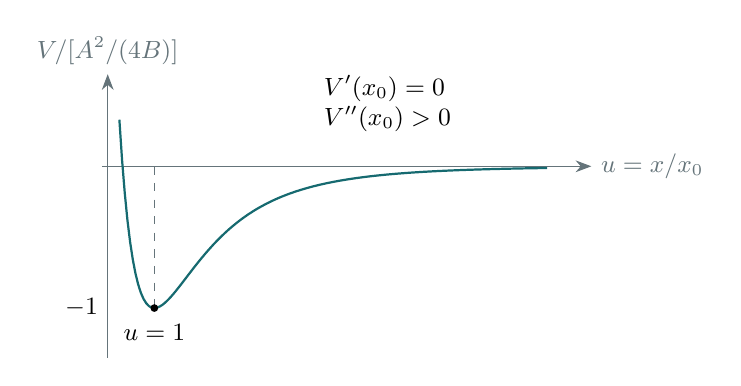
\begin{tikzpicture}[x=3.7cm,y=1.8cm,font=\small]
\draw[axis] (.82,0)--(2.5,0) node[right] {$u=x/x_0$};
\draw[axis] (.84,-1.35)--(.84,.65) node[above] {$V/[A^2/(4B)]$};
\draw[traj,domain=.88:2.35,samples=160] plot(\x,{pow(\x,-12)-2*pow(\x,-6)});
\draw[guide] (1,0)--(1,-1);\fill (1,-1) circle(1.4pt);
\node[below] at (1,-1.05) {$u=1$};\node[left] at (.84,-1) {$-1$};
\node[align=left] at (1.8,.44) {$V'(x_0)=0$\\$V''(x_0)>0$};
\end{tikzpicture}\figcaption{解图 热4.12B　势能极小确定平衡，势能曲率确定小形变刚度。}\end{minipage}\end{center}
\textbf{力控制下的断裂极限。} 准静态外力逐渐增加时，平衡满足$F_{\rm ext}=F(x)$，稳定要求$V''(x)>0$。在外拉力曲线最大值处$F'(x_m)=V''(x_m)=0$，有
\[
42Ax_m^6=156B,\qquad
x_m=\left(\frac{26B}{7A}\right)^{1/6}.
\]
继续增大拉力不再有稳定均匀的静态支，因此临界形变为
\[
\result{\varepsilon_m=\frac{x_m-x_0}{x_0}
=\left(\frac{13}{7}\right)^{1/6}-1=0.10868\simeq0.11}.
\]
相应极限拉力可写为$F_m=36A/(13x_m^7)$。这是最近邻、零温、均匀一维链且按外力加载的模型结果；实际缺陷、热涨落及不同加载约束都可能改变断裂。若链含$N_b$条相同串联键，整条链对总伸长的刚度为$k_{\rm bond}/N_b$，相同整体相对形变仍对应$F\simeq K\varepsilon$。
\subsubsection*{以无量纲力与势能逐点对应}
令$u=x/x_0$，利用$B=Ax_0^6/2$，完整势能和外拉力可写成
\[
\frac{V(x)}{A^2/(4B)}=u^{-12}-2u^{-6},\qquad
\frac{F(x)}{6A/x_0^7}=u^{-7}-u^{-13}.
\]
解图热4.12A、B分别按这两个函数绘制，
$u=1$在势能极小点也在外拉力零点，
$u=(13/7)^{1/6}$在外拉力峰值也在势能拐点。
外拉力的归一化斜率在$u=1$等于6，
图A的小形变切线因此是$F/(6A/x_0^7)=6(u-1)$。
切线给谷底处的局部斜率。力的峰值用完整力曲线求，分离功用同一完整曲线积分。

小形变展开的常数项消失是因为
$6A/x_0^7=12B/x_0^{13}$，
两个一次项的系数分别为$-7$与$+13$，相加才得6。
因此$F\simeq(36A/x_0^8)\Delta x$与
$F\simeq(36A/x_0^7)\varepsilon$对应以伸长量和相对形变为自变量的同一条局部力律。
若链有$N_b$条均匀串联键，能量二阶增量为
\[
\Delta E=\frac12N_b k_{\rm bond}(\Delta x)^2
=\frac12\frac{k_{\rm bond}}{N_b}(\Delta L)^2,
\qquad\Delta L=N_b\Delta x.
\]
能量式直接给整链对总伸长的刚度。若给链规定有效截面积 $S$，以应力除以应变得到的模量为 $K/S$。

\subsubsection*{外力做功、有效势与断裂判据}
固定拉力 $F_{\rm ext}$ 时，取有效势
$\Phi(x)=V(x)-F_{\rm ext}x$。
平衡由$\Phi'=0$给出，稳定由$\Phi''=V''>0$给出；
拉力增加到峰值时，稳定极小点与不稳定极大点合并，
继续增力便不存在相邻的稳定均匀静态支。
自由势能 $V$ 在整个拉伸支上持续升高并趋向零。稳定点合并发生在力的峰值，即 $V$ 的拐点。

把$B=7Ax_m^6/26$代入完整力，
\[
F_m=\frac{6A}{x_m^7}-\frac{12}{x_m^{13}}\frac{7Ax_m^6}{26}
=\frac{36A}{13x_m^7}.
\]
准静态把单键从$x_0$完全拆到无穷远所需净功为
\[
W_{\rm sep}=\int_{x_0}^{\infty}F(x)\dd x
=V(\infty)-V(x_0)=\frac{A^2}{4B}.
\]
分离功包含从力峰到无穷远的功，单位是焦耳。力控制下约 $10.87\%$ 的应变则是均匀稳定支终点的位置。多键链若只固定总长度，键长仍可相互补偿地变化；稳定性取决于 $\sum_i V''(x_i)(\delta x_i)^2$ 在 $\sum_i\delta x_i=0$ 的扰动下的符号。单键的间距被直接固定时，相对坐标由支承确定。


\Needspace{18\baselineskip}

\pdfbookmark[2]{第 13 题 NaCl晶体结合能的估算}{q13}

\section*{第 13 题\quad NaCl晶体结合能的估算}

NaCl晶体平衡时最近邻异号离子距离$r_0=2.81\times10^{-10}\,\mathrm m$，绝热压缩系数$k_s=3.3\times10^{-11}\,\mathrm{Pa^{-1}}$，马德隆常量$\alpha_M=1.75$。采用每个离子对势能$u(r)=B/r^n-\alpha_M e^2/(4\pi\varepsilon_0r)$的库仑吸引与幂次排斥模型，晶体体积$V=2Nr^3$，热运动能量对弹性和结合能的影响忽略。求1 mol NaCl的平衡势能$E_{p0}$及把晶体拆成孤立离子所需的结合能大小。

\begin{center}\begin{minipage}{0.96\linewidth}\centering\begin{tikzpicture}[x=1cm,y=1cm,font=\small,every node/.append style={align=center}]\foreach \i in {0,1,2,3}{\foreach \j in {0,1,2,3}{\pgfmathtruncatemacro{\parity}{mod(\i+\j,2)}
\ifnum\parity=0 \node[draw,circle,fill=blue!12,inner sep=3pt] at(\i,\j){$+$};\else\node[draw,circle,fill=brown!12,inner sep=3pt] at(\i,\j){$-$};\fi}}
\draw[<->] (0,-.6)--(1,-.6) node[midway,below]{$r_0$};\node[right] at (3.7,1.5){交替离子截面\\库仑项与排斥项};\end{tikzpicture}\figcaption{图 热4.13　马德隆常量计入整个晶格的静电作用。}\end{minipage}\end{center}

\Needspace{8\baselineskip}\subsection*{解答}

短程排斥势的指数记为 $n>1$。记$C=\alpha_Me^2/(4\pi\varepsilon_0)$。$N$个NaCl离子对的势能为
\[
E_p(r)=N\left(\frac B{r^n}-\frac Cr\right).
\]
第一项排斥为正，第二项吸引为负；分离离子的势能零点取在无穷远。

\textbf{平衡消去排斥系数。} $E_p'(r_0)=0$给
\[
-\frac{nB}{r_0^{n+1}}+\frac C{r_0^2}=0,
\quad B=\frac Cn r_0^{n-1}.
\]
于是平衡势能为
\[
E_{p0}=\frac{NC}{r_0}\left(\frac1n-1\right)<0.
\]
还需用压缩系数确定$n$。在忽略热运动能量的模型中，绝热内能改变近似等于$\dd E_p=-p\dd V$，故
\[
p=-\frac{\dd E_p}{\dd V},\qquad
\frac1{k_s}=-V\frac{\dd p}{\dd V}=V\frac{\dd^2E_p}{\dd V^2}.
\]
\begin{center}\begin{minipage}{0.96\linewidth}\centering\begin{tikzpicture}[x=1cm,y=1cm,font=\small,every node/.append style={align=center}]\draw[object] (0,0) rectangle(2,2);\draw[object] (0,2)--(.7,2.7)--(2.7,2.7)--(2,2);
\draw[object] (2,0)--(2.7,.7)--(2.7,2.7);\draw[guide] (0,0)--(.7,.7)--(2.7,.7);\draw[guide] (.7,.7)--(.7,2.7);
\draw[<->] (0,-.5)--(2,-.5) node[midway,below]{$2r$};\node[right] at(3,1.5){常规立方晶胞含4个离子对\\$V_{\rm cell}=(2r)^3$\\每离子对体积$2r^3$};\end{tikzpicture}\figcaption{解图 热4.13A　NaCl的两种离子分别构成面心立方子晶格。}\end{minipage}\end{center}
解图热4.13A中，晶胞边长是最近邻异号离子间距的两倍，即$2r$；每个晶胞包含4个NaCl离子对。因此$N$个离子对占$N/4$个晶胞，总体积为$(N/4)(2r)^3=2Nr^3$。均匀压缩时晶胞体积与 $r^3$ 同比变化。

\textbf{把体积导数改写成间距导数。} NaCl常规立方晶胞边长$2r$，含4个离子对，故$V=2Nr^3$，并有
\[
\frac{\dd r}{\dd V}=\frac1{6Nr^2}.
\]
链式求导保留两项：
\[
\frac{\dd^2E_p}{\dd V^2}
=E_p''(r)\left(\frac{\dd r}{\dd V}\right)^2
+E_p'(r)\frac{\dd^2r}{\dd V^2}.
\]
只在平衡点，第二项因$E_p'(r_0)=0$消失。因此
\[
\frac1{k_s}=\frac{E_p''(r_0)}{18Nr_0}.
\]
再计算并代入已消元的$B$：
\begin{align*}
E_p''(r_0)&=N\left[\frac{n(n+1)B}{r_0^{n+2}}-\frac{2C}{r_0^3}\right]\\
&=\frac{NC}{r_0^3}[(n+1)-2]=\frac{N(n-1)C}{r_0^3}.
\end{align*}
所以
\[
\frac1{k_s}=\frac{(n-1)C}{18r_0^4},\qquad
\result{n=1+\frac{18r_0^4}{k_sC}}.
\]
用$e=1.602176634\times10^{-19}\,\mathrm C$、$\varepsilon_0=8.85419\times10^{-12}\,\mathrm{F/m}$、$N_A=6.02214076\times10^{23}\,\mathrm{mol^{-1}}$，有
\[
C=4.03739\times10^{-28}\,\mathrm{J\cdot m},\quad n=9.4233,
\quad\frac{N_AC}{r_0}\simeq8.65\times10^5\,\mathrm{J/mol}.
\]
从而
\[
\result{E_{p0}=-7.73\times10^5\,\mathrm{J/mol}}.
\]
分离后，离子彼此远离，势能为零。系统的势能变化为 $0-E_{p0}$，故拆成孤立离子所需的结合能大小为 $7.73\times10^5\,\mathrm{J/mol}$，约 $0.77\,\mathrm{MJ/mol}$。正值对应拆散时对系统输入的功。
\subsubsection*{晶胞计数与平衡点的压力斜率}
解图热4.13A中可把一种离子的晶胞计数写为
$8\times\frac18+6\times\frac12=4$，
另一种写为$12\times\frac14+1=4$，
所以每个边长2r的常规晶胞共含8个离子，即4个NaCl离子对。
马德隆常量给出每个离子对的库仑能量，已经计入晶格中各离子的相互作用和成对计数。晶体含$N$个离子对，故库仑能量为$-NC/r$。
单个离子的平均能量是每离子对能量的一半，摩尔NaCl则包含$N_A$个离子对。

由$\dd V/\dd r=6Nr^2$，完整压力函数为
\[
p(r)=-\frac{E_p'(r)}{6Nr^2}
=\frac16\left(\frac{nB}{r^{n+3}}-\frac C{r^4}\right).
\]
使用平衡消元式后，直接对r求导，再用$\dd r/\dd V$转回体积导数，
在平衡点的斜率来自两个幂项的导数之差，$n+3-4=n-1$，从而 $-V(\dd p/\dd V)_0=(n-1)C/(18r_0^4)$。
其中压力的正号对应压缩，膨胀支在这个静态模型内需外部拉应力维持。
在任意$r$处，体积二阶导数还包含径向一阶导数与$\dd^2r/\dd V^2$的乘积：
\[
\frac{\dd^2r}{\dd V^2}=-\frac1{18N^2r^5},\qquad
\frac{\dd^2E_p}{\dd V^2}
=\frac{E_p''(r)}{36N^2r^4}-\frac{E_p'(r)}{18N^2r^5}.
\]
只在零外压的平衡点$E_p'(r_0)=0$，后一项才消失。

\begin{center}\begin{minipage}{.96\linewidth}\centering
\begin{tikzpicture}[x=30cm,y=15cm,font=\small]
\draw[axis] (.93,0)--(1.08,0) node[right] {$v=V/V_0$};
\draw[axis] (.94,-.09)--(.94,.115) node[above] {$p/B_{s0}$};
\draw[traj,domain=.95:1.06,samples=100] plot(\x,{3/8.4233*(pow(\x,-12.4233/3)-pow(\x,-4/3))});
\draw[warm,dashed,thick,domain=.95:1.06] plot(\x,{1-\x});
\node[below] at (1,0) {$1$};\node at (1.025,.08) {虚线$1-v$};
\foreach \v in {.96,1.04}{\draw(\v,-.002)--(\v,.002) node[below=3pt] {$\v$};}
\foreach \p in {-.05,.05}{\draw(.939,\p)--(.941,\p) node[left=3pt] {$\p$};}
\end{tikzpicture}
\figcaption{解图 热4.13B　完整静态压力与平衡点切线，$B_{s0}=1/k_s$。}
\end{minipage}\end{center}
解图热4.13B的斜率在$v=1$为负1，
表示$p\simeq-B_{s0}\Delta V/V_0$，体积减少时压力增加。
曲线以$n\simeq9.4233$作图，纵轴按零压平衡点的体积模量$B_{s0}=1/k_s$归一化。
量纲上C为J乘m，$r_0^4/(k_sC)$无量纲；
$N_AC/r_0$则为每摩尔能量，最后的正拆散功约为0.773 MJ/mol。

热运动总能量和结合能绝对值相差较大。热压的大小及其对体积的导数则由热能随体积的变化决定。本题另取静态近似，把给定绝热模量主要归于晶格势能的曲率。若要分开等温和绝热弹性、热膨胀及晶格振动的贡献，需要热膨胀系数、热容量等相应热力学数据。


\Needspace{18\baselineskip}

\pdfbookmark[2]{第 14 题 等温压缩氟利昂的液化质量}{q14}

\section*{第 14 题\quad 等温压缩氟利昂的液化质量}

质量$M=2.0\,\mathrm{kg}$的氟利昂在$-13{}^\circ\mathrm{C}$下由$V_i=0.19\,\mathrm{m^3}$等温压缩至$V_f=0.10\,\mathrm{m^3}$。摩尔质量$\mu=121\times10^{-3}\,\mathrm{kg/mol}$，该温度液体密度$\rho_l=1.44\times10^3\,\mathrm{kg/m^3}$，饱和蒸汽压$p_s=2.08\times10^5\,\mathrm{Pa}$。饱和蒸汽视为理想气体。求压缩中液化的质量；先检查初态是否已有液体，保留终态液体所占体积。

\begin{center}\begin{minipage}{0.96\linewidth}\centering\begin{tikzpicture}[x=1cm,y=1cm,font=\small,every node/.append style={align=center}]\draw[object] (0,0) rectangle(2.3,2.8);\draw[object,very thick] (0,2.5)--(2.3,2.5);\node at(1.15,1.3){初态\\$V_i=0.19$};
\draw[motion] (2.7,1.4)--(3.7,1.4);\draw[object] (4.2,0) rectangle(6.5,2.8);\draw[object,very thick] (4.2,1.9)--(6.5,1.9);
\fill[blue!18] (4.2,0) rectangle(6.5,.5);\node at(5.35,1.2){饱和蒸汽};\node at(5.35,.25){液体};\node[below] at(3.2,-.4){全程$T=260.15\,\mathrm K$};\end{tikzpicture}\figcaption{图 热4.14　气、液两相共同占据终态体积。}\end{minipage}\end{center}

\Needspace{8\baselineskip}\subsection*{解答}

先由总体积判断初态的相态。若2.0 kg全部为气体，初压为
\[
p_i=\frac{MRT}{\mu V_i},\qquad T=273.15-13=260.15\,\mathrm K.
\]
代入得$p_i=1.88169\times10^5\,\mathrm{Pa}<p_s$，故初态未达到饱和，没有液态氟利昂。刚开始液化的总体积为
\[
V_c=\frac{MRT}{\mu p_s}=0.171886\,\mathrm{m^3}.
\]
实际终体积$0.10\,\mathrm{m^3}$小于$V_c$且大于$M/\rho_l$，因此终态有两相。
\begin{center}\begin{minipage}{0.96\linewidth}\centering\begin{tikzpicture}[x=4.6cm,y=2.1cm,font=\small]
\draw[axis] (.25,0)--(1.3,0) node[right] {$v=V/V_c$};
\draw[axis] (.3,0)--(.3,1.4) node[above] {$p/p_s$};
\draw[traj] (.38,1)--(1,1);
\draw[traj,domain=1:1.18,samples=70] plot(\x,{1/\x});
\draw[guide] (1,0) node[below] {$1$}--(1,1);
\draw[guide] (.58178,0) node[below] {$V_f/V_c$}--(.58178,1);
\fill (1.10538,.90467) circle(1.4pt) node[right] {初态};
\node[left] at (.3,1) {$1$};
\draw[motion] (.85,1.16)--(.62,1.16) node[midway,above] {压缩};
\end{tikzpicture}\figcaption{解图 热4.14A　先在全气态支压缩，达到饱和压强后继续液化。}\end{minipage}\end{center}
解图热4.14A中从右向左压缩：先沿全气态支到达$V_c$，随后在饱和压强$p_s$的平台上液化。图中终体积$V_f<V_c$，所以要把终态总体积分成液体和蒸汽两部分；蒸汽状态方程使用$V_f-m_l/\rho_l$，剩余的 $m_l/\rho_l$ 是液体体积。

设终态液体质量为$m_l$、蒸汽质量为$m_g=M-m_l$。液体体积$m_l/\rho_l$，所以蒸汽体积$V_g=V_f-m_l/\rho_l$。在共存态蒸汽压强为$p_s$，有
\[
p_s\left(V_f-\frac{m_l}{\rho_l}\right)
=\frac{M-m_l}{\mu}RT.
\]
展开并收集$m_l$，
\[
m_l\left(\frac{RT}{\mu}-\frac{p_s}{\rho_l}\right)
=\frac{MRT}{\mu}-p_sV_f,
\]
故
\Needspace{11\baselineskip}
\[
\result{m_l=\frac{MRT/\mu-p_sV_f}{RT/\mu-p_s/\rho_l}=0.84325\,\mathrm{kg}\simeq0.84\,\mathrm{kg}}.
\]
初态没有液体，故此数值全是在压缩过程中新液化的质量。终态液体体积约$5.86\times10^{-4}\,\mathrm{m^3}$，蒸汽质量约1.157 kg，仍有大量气相。

若忽略液体体积，式子会给$m_l\simeq M-p_s\mu V_f/(RT)=0.83643\,\mathrm{kg}$，相差约0.007 kg；题设给出液体密度，因此保留这一修正。公式只适用于气液共存：当$V_f\ge V_c$时液化质量为零；当 $V_f=M/\rho_l$ 时 $m_l=M$，蒸汽体积趋于零。随后若继续压缩，压力由纯液体的压缩关系决定。
\subsubsection*{两相密度与液体质量}
在给定温度，饱和蒸汽密度为
\[
\rho_v=\frac{p_s\mu}{RT}\simeq11.6357\,\mathrm{kg/m^3}.
\]
初态平均密度$M/V_i\simeq10.526\,\mathrm{kg/m^3}$小于饱和蒸汽密度，
所以初态为未饱和气体；终态平均密度20 $\mathrm{kg/m^3}$处于$\rho_v$与$\rho_l$之间，允许气液共存。
相同结论也由$M/\rho_l<V_f<M/\rho_v=V_c$得到。

两相质量及体积守恒写成
$M=m_l+\rho_v(V-m_l/\rho_l)$，解得
\[
m_l(V)=\frac{M-\rho_vV}{1-\rho_v/\rho_l},\qquad
\frac{\dd m_l}{\dd V}=-\frac{\rho_v}{1-\rho_v/\rho_l}.
\]
在同温共存区，气液密度均固定，液体质量随总体积线性下降。
若初态已经在共存区，新增液化量应取
\[
\Delta m_l=\frac{\rho_v(V_i-V_f)}{1-\rho_v/\rho_l},
\]
本题由全气态压至两相，体积从 $V_i$ 缩到 $V_c$ 时仍无液体。平台段的体积变化为 $V_c-V_f$，代入同一斜率得到过程新增液体质量。

\begin{center}\begin{minipage}{.96\linewidth}\centering
\begin{tikzpicture}[x=29cm,y=1.25cm,font=\small]
\draw[axis] (0,0)--(.213,0) node[right] {$V/\mathrm{m^3}$};
\draw[axis] (0,0)--(0,2.5) node[above] {$m_l/\mathrm{kg}$};
\draw[traj] (.001388889,2)--(.171886,0);
\draw[guide] (.171886,0)--(.19,0);
\draw[guide] (.1,0) node[below] {$0.10$}--(.1,.84325)--(0,.84325) node[left] {$0.843$};
\node[above right] at (.171886,0) {$V_c$};\node[left] at (0,2) {$2$};
\node at (.075,2.25) {共存区为直线};
\end{tikzpicture}
\figcaption{解图 热4.14B　终态液体质量取在共存直线上，初态尚位于右侧全气体区。}
\end{minipage}\end{center}
解图热4.14B的液体全质量端点是$V=M/\rho_l\simeq0.001389\,\mathrm{m^3}$，
当前终点离纯液端还有约 $0.0986\,\mathrm{m^3}$，终态容器的大部分空间仍由蒸汽占据。
忽略液体体积会把上式分母近似成1；
误差的小参数是$\rho_v/\rho_l\simeq0.00808$，
它也等于这一近似相对完整液化质量的偏小比例，约0.81\%。

若另取准静态等温压缩，外界对流体的功可以按解图热4.14A分段计算：
\[
W_{\rm on}=\frac M\mu RT\ln\frac{V_i}{V_c}+p_s(V_c-V_f).
\]
第一段为理想气体等温压缩，第二段为两相平台的恒压压缩。
气相等温段的理想气体内能不变，放热等于该段外功。在两相段，外功与汽液内能差共同决定放热。
若另给该温度每千克的汽化焓L，平台段放热为$m_lL$，
总放热为$(M/\mu)RT\ln(V_i/V_c)+m_lL$。
等温过程中液相质量改变，整个两相流体的内能仍会变化。


\Needspace{18\baselineskip}

\pdfbookmark[2]{第 15 题 互不相溶液体共沸温度与蒸汽组成}{q15}

\section*{第 15 题\quad 互不相溶液体共沸温度与蒸汽组成}

互不相溶液体A、B的饱和蒸汽压满足$\ln(p_i/p_0)=a_i/T+b_i$，$T$用绝对温标，$p_0$为标准大气压。测得数据：
\begin{center}\begin{tabular}{ccc}\toprule 温度 & $p_A/p_0$ & $p_B/p_0$\\\midrule40℃&0.284&0.07278\\90℃&1.476&0.6918\\\bottomrule\end{tabular}\end{center}
外压为$p_0$，先求A、B各自沸点。再将100 g A、100 g B置于图示容器，在B上方覆盖不挥发、与A和B均不相溶的薄液层C，抑制B在自由液面的蒸发；各层静水压忽略。A、B蒸汽在界面气泡中混合，服从道尔顿分压定律，摩尔质量比$\mu_A/\mu_B=8$。持续缓慢加热，温度图有两段平台。求第一、第二平台温度$t_1,t_2$（到1℃），及图中第一平台结束、升温至第二平台的阶段内$\tau_1$时刻两液体剩余质量（到0.1 g）。气相滞留量及非沸腾阶段的自由蒸发损失忽略。

\begin{center}\begin{minipage}{0.96\linewidth}\centering\begin{tikzpicture}[x=1cm,y=1cm,font=\small,every node/.append style={align=center}]\draw[object] (0,0) rectangle(2.4,3);\fill[blue!18] (0,0) rectangle(2.4,1);\fill[brown!18] (0,1) rectangle(2.4,2);
\fill[gray!18] (0,2) rectangle(2.4,2.3);\node at(1.2,.5){A};\node at(1.2,1.5){B};\node at(1.2,2.15){C};
\draw[motion] (1.2,1)--(1.2,2.8) node[above]{混合气泡};
\draw[axis] (3.5,0)--(8.5,0) node[right]{$\tau$};\draw[axis] (3.5,0)--(3.5,3.3) node[above]{$t$};
\draw[traj] (3.6,.2)--(4.6,1.1)--(6.1,1.1)--(7.3,2.6)--(8.2,2.6);
\node[left] at(3.5,1.1){$t_1$};\node[left] at(3.5,2.6){$t_2$};\draw[guide] (6.65,0) node[below]{$\tau_1$}--(6.65,1.8);\end{tikzpicture}\figcaption{图 热4.15　A、B共同沸腾形成第一平台，剩余液体形成第二平台。}\end{minipage}\end{center}

\Needspace{8\baselineskip}\subsection*{解答}

解图热4.15A比较两种饱和蒸汽压及其和，用压强和达到外压确定共同沸点；解图热4.15B再按蒸汽组成计算两种液体的质量损失。

拟合横坐标使用绝对温度的倒数，取 $T_{40}=313.15\,\mathrm K$、$T_{90}=363.15\,\mathrm K$。对每一种液体，两次测量相减给
\[
a_i=\frac{\ln[p_i(40)/p_0]-\ln[p_i(90)/p_0]}{1/T_{40}-1/T_{90}},\quad
b_i=\ln[p_i(40)/p_0]-\frac{a_i}{T_{40}}.
\]
数据代入得到
\begin{center}\begin{tabular}{ccc}\toprule 液体 &$a_i/\mathrm K$ &$b_i$\\\midrule
A&$-3748.4907$&10.711491\\B&$-5121.6396$&13.734914\\\bottomrule\end{tabular}\end{center}
\textbf{各自沸点。} 外压为$p_0$时纯液体沸腾条件是$p_i=p_0$，故$a_i/T_{bi}+b_i=0$。于是
\[
T_{bA}=-a_A/b_A=349.9504\,\mathrm K,\quad t_{bA}=76.8004{}^\circ\mathrm{C}\simeq77{}^\circ\mathrm{C},
\]
\[
T_{bB}=-a_B/b_B=372.8920\,\mathrm K,\quad t_{bB}=99.7420{}^\circ\mathrm{C}\simeq100{}^\circ\mathrm{C}.
\]
\begin{center}\begin{minipage}{0.96\linewidth}\centering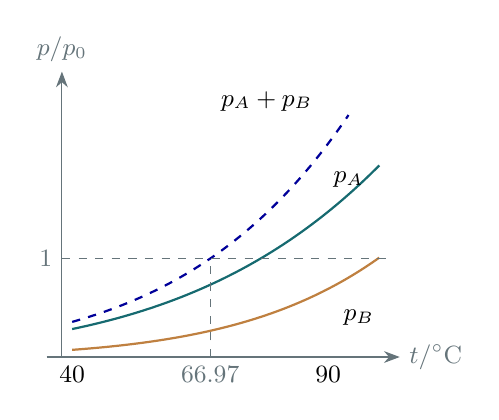
\begin{tikzpicture}[x=.065cm,y=1.25cm,font=\small]
\draw[axis] (35,0)--(104,0) node[right] {$t/{}^\circ\mathrm C$};
\draw[axis] (38,0)--(38,2.9) node[above] {$p/p_0$};
\draw[traj,domain=40:100,samples=120] plot(\x,{exp(-3748.490701449689/(273.15+\x)+10.711491037894)});
\draw[brown,thick,domain=40:100,samples=120] plot(\x,{exp(-5121.639642083960/(273.15+\x)+13.734913893671)});
\draw[blue!60!black,thick,dashed,domain=40:94,samples=120] plot(\x,{exp(-3748.490701449689/(273.15+\x)+10.711491037894)+exp(-5121.639642083960/(273.15+\x)+13.734913893671)});

\draw[guide] (38,1) node[left] {$1$}--(102,1);
\draw[guide] (66.97083,0) node[below] {$66.97$}--(66.97083,1);
\foreach \t in {40,90}{\node[below] at (\t,0) {$\t$};}
\node at (78,2.6) {$p_A+p_B$};\node at (94,1.8) {$p_A$};\node at (96,.4) {$p_B$};
\end{tikzpicture}\figcaption{解图 热4.15A　两种饱和蒸汽压之和先达到外压。}\end{minipage}\end{center}
\textbf{第一平台。} 图中界面气泡同时含A、B蒸汽；两液体互不相溶且都尚未耗尽，各自分压为相应饱和蒸汽压。沸腾条件为
\[
p_A(T_1)+p_B(T_1)=p_0,
\quad Y(t)=e^{a_A/(273.15+t)+b_A}+e^{a_B/(273.15+t)+b_B}=1.
\]
两项随温度单调增加，故根唯一。用未提前舍入的参数作数值夹逼：
\begin{center}\begin{tabular}{cc}\toprule $t/{}^\circ\mathrm{C}$ & $Y(t)$\\\midrule
40&0.35678\\59&约0.749\\66&约0.966\\66.5&约0.984\\67&约1.001\\70&约1.113\\90&2.1678\\\bottomrule\end{tabular}\end{center}
继续夹逼得$T_1=340.12083\,\mathrm K$，即
\[
\result{t_1=66.9708{}^\circ\mathrm{C}\simeq67{}^\circ\mathrm{C}}.
\]
根处$p_A=0.733766p_0$、$p_B=0.266234p_0$，和正好为$p_0$。第一平台低于两种纯液体沸点，因为此时两分压共同支承外压。

\textbf{平台期间的质量损失。} 取一个温度$T_1$、体积$V$的混合气泡，两种气体占同一体积，分别满足
\[
p_AV=\frac{m_A}{\mu_A}RT_1,\quad p_BV=\frac{m_B}{\mu_B}RT_1.
\]
因此蒸汽质量比，也是两液体在共沸平台上的损失质量比，为
\[
\frac{\dd m_{A,\rm loss}}{\dd m_{B,\rm loss}}
=\frac{\mu_Ap_A}{\mu_Bp_B}
=8\frac{0.733766}{0.266234}=22.0488.
\]
两蒸汽的分压比是 $2.756$，即同一气泡中两种气体的摩尔数之比；乘上摩尔质量比8才得到气泡带走的质量比。两者初始均100 g，A先耗尽。A失去100 g时，B只失去$100/22.0488=4.53540\,\mathrm g$。
\begin{center}\begin{minipage}{0.96\linewidth}\centering\begin{tikzpicture}[x=1cm,y=1cm,font=\small,every node/.append style={align=center}]\node[draw] (a) at(0,1.4){A：100 g};\node[draw] (b) at(4,1.4){B：100 g};
\draw[motion] (a)--(0,-.4) node[below]{损失100 g，耗尽};\draw[motion] (b)--(4,-.4) node[below]{损失4.5354 g};
\node at(2,2.5){$\dd m_A/\dd m_B=8p_A/p_B=22.0488$};\node at(2,-1.4){第一平台结束：A为0，B为95.4646 g};\end{tikzpicture}\figcaption{解图 热4.15B　共同沸腾时，两种液体的质量按气泡组成的比例减少。}\end{minipage}\end{center}
\textbf{第二平台与指定时刻。} A耗尽后共沸条件不再成立。剩余B在$t_1$下的蒸汽压小于外压，沸腾停止，继续加热使温度升到B自己的沸点，故
\[
\result{t_2=t_{bB}=99.7420{}^\circ\mathrm{C}\simeq100{}^\circ\mathrm{C}}.
\]
图中的$\tau_1$在第一平台结束后的升温段；忽略这段非沸腾蒸发和气相滞留量，质量保持为
\[
\result{m_A(\tau_1)=0,\quad m_B(\tau_1)=95.4646\,\mathrm g\simeq95.5\,\mathrm g}.
\]
第一平台内温度固定，余量随累计蒸发量变化。题中的 $\tau_1$ 已离开第一平台。覆盖层 C 抑制 B 从自由表面蒸发，A、B 界面的气泡仍同时取得两种蒸汽。
\subsubsection*{饱和压拟合、共沸根与蒸汽组成}
拟合时同一液体的两式相减，消去截距b，
两次对数差除以$1/313.15-1/363.15$才给斜率a。
例如A的对数由$\ln0.284\simeq-1.25878$升至$\ln1.476\simeq0.38934$，
由于温度上升时$1/T$下降，斜率a应为负。
温度上升时$1/T$减小，乘负斜率$a$后$a/T+b$增大，因而纯液体饱和压上升。两点确定的拟合曲线分别通过40℃和90℃时的测量压强。

令$Y(T)=p_A(T)/p_0+p_B(T)/p_0$，其导数为
\[
\frac{\dd Y}{\dd T}
=\frac{-a_A}{T^2}e^{a_A/T+b_A}
+\frac{-a_B}{T^2}e^{a_B/T+b_B}>0.
\]
结合40℃时$Y<1$、90℃时$Y>1$，可先证明这个区间有且仅有一个共沸根，
再用二分法或其他保持区间的数值法逼近。
在纯A沸点，A自己的分压已等于外压，而B的饱和分压仍正，故压强和超过外压；
纯B沸点同理，所以共沸温度严格低于两个纯液体沸点。
解图热4.15A用完整拟合函数绘制，压强和在约66.97℃穿过1，
两条单组分曲线在更高温度分别穿过1。
将两条$\ln p$拟合式取指数得到各自饱和压，再按道尔顿定律将两压强相加。

两液相互不相溶时，各自的液面分别与蒸汽平衡。只要两液相都在，各分压就由温度确定，第一平台温度和蒸汽组成保持固定。初始的100 g比100 g给出液体质量，蒸汽质量比由摩尔质量和分压比决定。若是均匀混合的液相，则另写含液相组成的平衡关系。
在同一个气泡中，理想气体分子共享同一V和T，
所以摩尔比为$p_A/p_B\simeq2.756$，质量比还要乘8，
A的气相摩尔分数约为 $73.38\%$。由于每摩尔A的质量是B的8倍，A的蒸汽质量分数达到 $95.66\%$。

\subsubsection*{将平台质量变化积分到一相耗尽}
令z为第一平台上B累计损失的质量，以g计，则A累计损失为qz，
其中$q=22.0488$在两液相都存在时保持常量。
剩余质量沿解图热4.15B的过程满足
\[
m_A=100-qz,\qquad m_B=100-z,\qquad
0\le z\le\min(100,100/q).
\]
只要两液体均存在，各气泡的组成都相同。将气泡带走的质量逐一相加，累计损失仍满足同一比例。
本题 $q>1$，沿解图热4.15B先到 $z=100/q$，此时A为零，B尚余 $100-100/q$。
一般初始质量为$m_{A0},m_{B0}$时，A先尽的条件为$m_{A0}/m_{B0}<q$；
等号时两者同时耗尽，不再有相同的第二液相平台。

A耗尽后，B在第一平台温度的饱和压只有约$0.266p_0$，
不足以维持对外沸腾，继续加热先使B和覆盖层升温。
到B自己的饱和压达到外压时才出现第二平台，
第二平台由尚存的B的纯液体饱和关系确定。
温度图中的两段斜线上，液体和容器吸收显热，斜率由净加热功率与热容量确定。若第一平台的净加热功率为恒量 $P$，两物质的单位质量汽化焓为 $L_A,L_B$，以质量的千克数代入 $P\Delta\tau=m_{A0}L_A+(m_{A0}/q)L_B$，得到A耗尽所需时间。平台内部的累计损失随已供给的相变热增加。液相可以沿气泡通路分别与气相达到饱和，覆盖层C只抑制B自由表面处的额外损失。


\Needspace{18\baselineskip}

\pdfbookmark[2]{第 16 题 冰水水蒸气三相定容加热后的质量分配}{q16}

\section*{第 16 题\quad 冰水水蒸气三相定容加热后的质量分配}

密闭刚性容器内只有冰、水、水蒸汽，初态三相质量均为1 g，在三相点$t=0.01{}^\circ\mathrm{C}$、$p=4.58\,\mathrm{mmHg}$平衡。保持容积不变，缓慢输入热量$Q=0.255\,\mathrm{kJ}$。求终态三相质量的估计。升华热$L_s=2.83\,\mathrm{kJ/g}$，汽化热$L_v=2.49\,\mathrm{kJ/g}$；水蒸汽视为理想气体，取水、冰密度约$10^3,0.9\times10^3\,\mathrm{kg/m^3}$。先检查三相是否仍共存，再说明忽略凝聚相体积变化的误差。

\begin{center}\begin{minipage}{0.96\linewidth}\centering\begin{tikzpicture}[x=1cm,y=1cm,font=\small,every node/.append style={align=center}]\draw[object] (0,0) rectangle(5.5,3.2);\fill[blue!10] (0,0) rectangle(5.5,.5);
\filldraw[fill=gray!25] (.3,.15) rectangle(1.1,.85);\node at(3,2){水蒸汽1 g\\占绝大部分容积};
\node[below] at(.7,-.1){冰1 g};\node[below] at(3.8,-.1){水1 g};\draw[force] (6.5,1)--(5.5,1) node[midway,above]{$Q$};\end{tikzpicture}\figcaption{图 热4.16　容器刚性密闭，三相共存时温度和压强固定。}\end{minipage}\end{center}

\Needspace{8\baselineskip}\subsection*{解答}

三相共存时，系统温度和压强保持在三相点。先估算熔化潜热：
\[
L_f=L_s-L_v=2.83-2.49=0.34\,\mathrm{kJ/g}.
\]
若1 g冰全部熔化，至少需要约0.34 kJ。实际输入0.255 kJ，尚不足以耗尽冰，这一热量只熔化部分冰，终态可保持三相温度和压强。再用体积与内能方程求小修正。
\begin{center}\begin{minipage}{0.96\linewidth}\centering\begin{tikzpicture}[x=1cm,y=1cm,font=\small,every node/.append style={align=center}]\draw[object] (0,0) rectangle(5,1);\fill[blue!20] (0,0) rectangle(3.75,1);\node at(1.8,.5){熔化0.75 g};\node at(4.4,.5){余冰};
\draw[<->] (0,1.5)--(5,1.5) node[midway,above]{1 g冰全熔：0.340 kJ};
\draw[<->] (0,-.5)--(3.75,-.5) node[midway,below]{实际加热：0.255 kJ};\end{tikzpicture}\figcaption{解图 热4.16A　输入热量不足以熔尽冰，三相点约束继续成立。}\end{minipage}\end{center}
解图热4.16A比较的是同一份1 g冰的熔化能量，0.255 kJ只占全熔所需0.340 kJ的四分之三。图中未耗尽的冰保证三相点约束仍成立，输入热量主要改变各相质量；后面再用刚性容器的体积约束估算蒸汽质量的微小修正。

\textbf{定容对水蒸汽质量的约束。} 初态$p=4.58\,\mathrm{mmHg}\simeq610.6\,\mathrm{Pa}$，$T=273.16\,\mathrm K$。理想水蒸汽密度为
\[
\rho_v=\frac{\mu p}{RT}
\simeq\frac{0.018\times610.6}{8.31446\times273.16}
=4.84\times10^{-3}\,\mathrm{kg/m^3}.
\]
它约比水、冰的密度小$2\times10^5$倍。初态三者质量相同，故1 g水蒸汽体积约0.207 $\mathrm{m^3}$，冰、水各约$10^{-6}\,\mathrm{m^3}$。容器绝大部分被蒸汽占据。

三相点温度、压强不变，蒸汽密度不变；忽略凝聚相体积相对于蒸汽体积的变化，定容就使蒸汽质量近似不变，仍为1 g。因此热量几乎全用于冰变水：
\[
\Delta m_{i\to l}=Q/L_f=0.255/0.34=0.75\,\mathrm g.
\]
终态结果为
\[
\result{m_i\simeq0.25\,\mathrm g,\quad m_l\simeq1.75\,\mathrm g,\quad m_v\simeq1.00\,\mathrm g}.
\]
终态还有约四分之一克冰，也有液水和蒸汽，三相均存在。

\Needspace{11\baselineskip}\textbf{凝聚相缩小后的蒸汽增量。} 若冰、水密度分别900、1000 $\mathrm{kg/m^3}$，熔化0.75 g使凝聚相总体积减少约
\[
\Delta V_c\simeq0.75\times10^{-3}\left(\frac1{1000}-\frac1{900}\right)
=-8.3\times10^{-8}\,\mathrm{m^3}.
\]
这相应增加蒸汽体积，质量增加约$\rho_v(-\Delta V_c)=4.0\times10^{-10}\,\mathrm{kg}=4.0\times10^{-7}\,\mathrm g$，汽化热修正约$10^{-6}\,\mathrm{kJ}$。刚性外壁无功，而所给潜热是近似定压焓差；改为内能差还应扣$p\Delta v$。其熔化项为约$6.8\times10^{-8}\,\mathrm{kJ/g}$，也远小于所需估算精度。终态蒸汽质量在所求精度下仍记为 $1.00\,\mathrm g$。
\subsubsection*{保留小体积项时的三方程解}
令x为冰减少的质量，y为蒸汽增加的质量，统一用kg。
则水增加$x-y$，总质量自动保持不变。
在三相点定义比体积$v_i=1/\rho_i$、$v_l=1/\rho_l$、$v_v=1/\rho_v$，
刚性容器的体积方程为
\[
-xv_i+(x-y)v_l+yv_v=0,
\qquad y=\frac{v_i-v_l}{v_v-v_l}x.
\]
冰融化后体积减小，故$y>0$，只需极少量水再汽化来填补增加的气相体积。
冰的比体积较大，由质量 $x$ 的冰转成水时释放出 $x(v_i-v_l)$ 的空间，重新分配给少量水蒸汽。

刚性外壁无体积功，输入热量等于内能增量。
所给潜热为近似焓差，将其转为每kg内能差：
\[
u_l-u_i=L_f-p(v_l-v_i),\qquad
u_v-u_l=L_v-p(v_v-v_l).
\]
其中$L_f=3.40\times10^5$ J/kg、$L_v=2.49\times10^6$ J/kg。
以冰为参考内能零点，完整能量方程为
\[
Q=x(u_l-u_i)+y(u_v-u_l).
\]
将体积式的y代入得
\[
x=\frac{Q}{L_f-p(v_l-v_i)
+\dfrac{v_i-v_l}{v_v-v_l}[L_v-p(v_v-v_l)]}.
\]
三相点压力固定，整个体积变化又为零，
上述分母中的两项p贡献实际恰好抵消：
\[
x=\frac{Q}{L_f+\dfrac{v_i-v_l}{v_v-v_l}L_v},\qquad
y=\frac{v_i-v_l}{v_v-v_l}x.
\]
凝聚相体积缩小，蒸汽体积相应增大。将两者乘同一三相点压力，所得两项大小相等、符号相反，故总内能增量等于总焓增量。

取题设近似密度及$p\simeq610.6$ Pa，得
$(v_i-v_l)/(v_v-v_l)\simeq5.377\times10^{-7}$，
$x\simeq0.7499970$ g、$y\simeq4.03\times10^{-7}$ g。
于是三相质量约为
\[
m_i=0.2500030\,\mathrm g,\quad
m_l=1.7499966\,\mathrm g,\quad
m_v=1.0000004\,\mathrm g.
\]
它们都为正、总质量仍为3 g，并满足同温、同压和定容，
所以终态仍处在三相点。
计算多保留几位小数以显示各相质量修正的量级，最终有效数字由所用密度和潜热的精度决定。
若继续加热，冰的质量先降为零。此后的温度、压强与水汽质量由水汽两相的能量、总体积和饱和条件决定。


\Needspace{18\baselineskip}

\pdfbookmark[2]{第 17 题 地幔硅酸盐熔点随深度变化}{q17}

\section*{第 17 题\quad 地幔硅酸盐熔点随深度变化}

地幔固态硅酸盐的熔化潜热为单位质量的$L_m$，液、固密度比$\alpha=\rho_l/\rho_s$。$r$表示离地心的距离。结合静力平衡和克拉珀龙方程，求熔点$T_m$随$r$的变化率。先以一般重力加速度$g_r$表示，再在均匀密度地球模型中写成表面重力$g$、地球半径$R$的形式。上部地幔某处$T_m=1300{}^\circ\mathrm{C}$、$\alpha=0.9$、$L_m=10^5\,\mathrm{cal/kg}$，估算向地心深入1000 m后的熔点变化，取$g=9.80\,\mathrm{m/s^2}$、$1\,\mathrm{cal}=4.184\,\mathrm J$。

\begin{center}\begin{minipage}{0.96\linewidth}\centering\begin{tikzpicture}[x=1cm,y=1cm,font=\small]
\draw[object] (0,0) circle(1.45);
\fill[blue!18] (10:1.1) arc[start angle=10,end angle=30,radius=1.1]--(30:1.2) arc[start angle=30,end angle=10,radius=1.2]--cycle;
\draw[guide] (0,0)--(20:1.15) node[midway,above] {$r$};
\node[below left] at (0,0) {地心};
\draw[object,fill=blue!10] (4,-.7) rectangle(5.2,.7);
\draw[force] (2.5,0)--(4,0) node[midway,above] {$p(r)S$};
\draw[force] (6.5,0)--(5.2,0) node[midway,above] {$p(r+\dd r)S$};
\draw[force] (4.95,-.45)--(4.15,-.45) node[midway,below=4pt] {$\rho_sS\dd r\,g_r$};
\draw[<->] (4,1.1)--(5.2,1.1) node[midway,above] {$\dd r$};
\draw[axis] (3,-1.4)--(6.4,-1.4) node[right] {$r$向外};
\node at (4.6,1.8) {局部薄层受力};
\end{tikzpicture}\figcaption{图 热4.17　径向坐标向外增加，重力指向地心。}\end{minipage}\end{center}

\Needspace{8\baselineskip}\subsection*{解答}

先不指定地球密度分布。解图热4.17A给出熔点随深度变化的两种趋势，斜率的符号由熔化体积变化确定。图中径向坐标$r$向外增加，厚$\dd r$、面积$S$的地幔薄层受内侧较大的压力与向内的重力。静力平衡为
\[
[p(r)-p(r+\dd r)]S=\rho_sg_rS\dd r,
\qquad\frac{\dd p}{\dd r}=-\rho_sg_r.
\]
固液共存的克拉珀龙方程可由单位质量的吉布斯势相等求导得到：$-s_l\dd T+v_l\dd p=-s_s\dd T+v_s\dd p$，又$s_l-s_s=L_m/T_m$，所以
\[
\frac{\dd T_m}{\dd p}=\frac{T_m(v_l-v_s)}{L_m}.
\]
其中$v_l=1/(\alpha\rho_s)$、$v_s=1/\rho_s$，故
\[
v_l-v_s=\frac{1-\alpha}{\alpha\rho_s}.
\]
与静力梯度相乘，密度消去，得到一般表达式
\[
\result{\frac{\dd T_m}{\dd r}=\frac{\alpha-1}{\alpha}\frac{T_mg_r}{L_m}}.
\]
\begin{center}\begin{minipage}{0.96\linewidth}\centering\begin{tikzpicture}[x=4.7cm,y=.52cm,font=\small]
\draw[axis] (0,0)--(1.25,0) node[right] {$z/\mathrm{km}$};
\draw[axis] (0,-4.2)--(0,5.5) node[above] {$\Delta T_m/\mathrm K$};
\draw[traj] plot coordinates {(0.000000,0.000000000) (0.025000,0.102356673) (0.050000,0.204720006) (0.075000,0.307089999) (0.100000,0.409466653) (0.125000,0.511849968) (0.150000,0.614239945) (0.175000,0.716636584) (0.200000,0.819039885) (0.225000,0.921449848) (0.250000,1.023866476) (0.275000,1.126289766) (0.300000,1.228719721) (0.325000,1.331156341) (0.350000,1.433599626) (0.375000,1.536049576) (0.400000,1.638506192) (0.425000,1.740969474) (0.450000,1.843439423) (0.475000,1.945916039) (0.500000,2.048399323) (0.525000,2.150889275) (0.550000,2.253385895) (0.575000,2.355889184) (0.600000,2.458399143) (0.625000,2.560915771) (0.650000,2.663439070) (0.675000,2.765969039) (0.700000,2.868505680) (0.725000,2.971048992) (0.750000,3.073598975) (0.775000,3.176155632) (0.800000,3.278718961) (0.825000,3.381288963) (0.850000,3.483865639) (0.875000,3.586448989) (0.900000,3.689039014) (0.925000,3.791635714) (0.950000,3.894239089) (0.975000,3.996849140) (1.000000,4.099465867)};
\draw[brown,thick,dashed] plot coordinates {(0.000000,-0.000000000) (0.025000,-0.083741416) (0.050000,-0.167478374) (0.075000,-0.251210874) (0.100000,-0.334938918) (0.125000,-0.418662504) (0.150000,-0.502381633) (0.175000,-0.586096307) (0.200000,-0.669806523) (0.225000,-0.753512284) (0.250000,-0.837213589) (0.275000,-0.920910438) (0.300000,-1.004602833) (0.325000,-1.088290772) (0.350000,-1.171974256) (0.375000,-1.255653285) (0.400000,-1.339327860) (0.425000,-1.422997981) (0.450000,-1.506663649) (0.475000,-1.590324862) (0.500000,-1.673981622) (0.525000,-1.757633929) (0.550000,-1.841281783) (0.575000,-1.924925184) (0.600000,-2.008564133) (0.625000,-2.092198629) (0.650000,-2.175828674) (0.675000,-2.259454266) (0.700000,-2.343075407) (0.725000,-2.426692097) (0.750000,-2.510304336) (0.775000,-2.593912124) (0.800000,-2.677515461) (0.825000,-2.761114348) (0.850000,-2.844708785) (0.875000,-2.928298772) (0.900000,-3.011884310) (0.925000,-3.095465398) (0.950000,-3.179042037) (0.975000,-3.262614227) (1.000000,-3.346181968)};
\draw[guide] (1,-3.35)--(1,4.1);
\node[below right] at (1,0) {$1$};\node[left] at (0,4) {$4$};\node[left] at (0,-3) {$-3$};
\node at (.65,4.9) {$\alpha=0.9$};\node at (.65,-3.8) {$\alpha=1.1$};
\end{tikzpicture}\figcaption{解图 热4.17A　局部恒定重力示例：初熔点1573.15 K，熔化体积的正负决定温变方向。}\end{minipage}\end{center}
\textbf{均匀密度地球近似。} 若地球质量$M$均匀分布、半径为$R$，半径$r$内质量$M_r=M(r/R)^3$，因此
\[
g_r=\frac{GM_r}{r^2}=\frac{GMr}{R^3}=g\frac rR,
\quad\result{\frac{\dd T_m}{\dd r}=\frac{\alpha-1}{\alpha}\frac{T_m}{L_m}g\frac rR}.
\]
若$\alpha,L_m$还取常量，这个近似方程可积分为
\[
\ln\frac{T_m(r)}{T_m(r_0)}
=\frac{\alpha-1}{\alpha}\frac{g}{2RL_m}(r^2-r_0^2).
\]
在球对称但密度有径向变化的模型中，取半径 $r$ 内的质量 $M(r)$ 求 $g_r=GM(r)/r^2$，再用同一局部方程积分。

\textbf{向内1000 m的变化。} 上部地幔取 $r\simeq R$，所以在这一公里内用局部的 $g\simeq9.80\,\mathrm{m/s^2}$。向内位移为 $\Delta r=-1000\,\mathrm m$，初熔点用摄氏值加273.15，得 $T_{m0}=1573.15\,\mathrm K$。潜热换成SI单位，
\[
L_m=10^5\,\mathrm{cal/kg}=4.184\times10^5\,\mathrm{J/kg}.
\]
局部一阶估算
\begin{align*}
\Delta T_m&\simeq\frac{0.9-1}{0.9}\frac{1573.15}{4.184\times10^5}
\times9.80\times(-1000)\,\mathrm K\\
&=+4.0941\,\mathrm K\simeq+4℃.
\end{align*}
液态密度较低，熔化时体积增大，加压使熔点升高，故向内温差为正。绝对温度参与比例运算，而温差1 K与1℃相同。这一公里里的温升相对初温约为 $0.0026$。用初始绝对温度代替区间内变化的 $T_m$，给出题设状态附近约 $4.09\,\mathrm{K/km}$ 的局部温升。
\subsubsection*{相平衡斜率与薄层受力的中间步骤}
在相邻的固液共存状态，两相比吉布斯势相等，分别微分有
\[
-s_l\dd T_m+v_l\dd p=-s_s\dd T_m+v_s\dd p,
\quad (s_l-s_s)\dd T_m=(v_l-v_s)\dd p.
\]
熔化焓按每单位质量给出，故$L_m=T_m(s_l-s_s)$，
克拉珀龙式中的熵和体积同样按单位质量计。
本题的密度比是液比固，
$v_l-v_s=1/(\alpha\rho_s)-1/\rho_s$，
因此 $\alpha<1$ 对应熔化时体积增加。

题图热4.17的局部薄层内侧压力沿r正向，外侧压力和重力沿r负向。
压力差乘同一截面积S与质量$\rho_sS\dd r$乘重力相等，
约去S、除以$\dd r$并取薄层极限后，才得负的径向压强梯度。
若取向内深度$z=R-r$作自变量，此时 $\dd r=-\dd z$，所以
\[
\frac{\dd T_m}{\dd z}
=\frac{1-\alpha}{\alpha}\frac{T_mg_{R-z}}{L_m}.
\]
解图热4.17A的$\alpha=0.9$曲线因此向上，
而$\alpha=1.1$曲线向下；两条曲线共享随深度增大的压力。两相比体积差改变符号，使压强升高时的熔点响应反向。

\subsubsection*{一般重力场的积分与局部误差}
若$\alpha,L_m$近似为常量，定义引力势满足$\dd\Phi/\dd r=g_r$，
一般式可积分为
\[
\ln\frac{T_m(r)}{T_m(r_0)}
=\frac{\alpha-1}{\alpha L_m}[\Phi(r)-\Phi(r_0)].
\]
均匀球的 $g_r=gr/R$ 在半径积分中给 $r^2-r_0^2$。一般球对称分布中，半径 $r$ 外各球壳的引力在该点相消，势差可由内部质量函数决定的 $g_r$ 积出。

\Needspace{20\baselineskip}
若只考虑局部g不变、初始温度为$T_{m0}$的深度区间d，
可先不把T在右边固定，得到
\[
T_m(d)=T_{m0}\exp\left[\frac{1-\alpha}{\alpha}\frac{gd}{L_m}\right].
\]
本题指数约0.002603，完整局部指数式给温升约4.10 K，
一阶式为4.0941 K，两者只差约0.0053 K。
差值来自将指数展开保留到一次项。这里在所取区间内把 $g,\alpha,L_m$ 视为常量。
均匀球从$r_0=R$向内d时，指数中的gd应改为$g[d-d^2/(2R)]$，
其额外相对修正尺度为$d/(2R)$，小深度时可以检查后略去。

局部公式中固态密度消去，是因为同一$\rho_s$同时进入岩石静力梯度与该物质的相变比体积。
若夹杂物在密度为 $\rho_{\rm host}$ 的宿主介质中熔化，压力梯度改为 $-\rho_{\rm host}g_r$，夹杂物的比体积差仍含 $1/\rho_s$，相乘后保留因子 $\rho_{\rm host}/\rho_s$。跨越较大温压区间时，可在微分方程内使用随位置或状态变化的 $L_m$ 和 $\alpha$。


\end{document}
